%%%%%%%%%%%%%%%%%%%%%%%%%%%%%%%%%%%%%%%%%%%%%%%%%%%%%%%%%%%%%%%%%%%%%%%%

%%% LaTeX Template for AAMAS-2023 (based on sample-sigconf.tex)
%%% Prepared by the AAMAS-2023 Program Chairs based on the version from AAMAS-2022. 

%%%%%%%%%%%%%%%%%%%%%%%%%%%%%%%%%%%%%%%%%%%%%%%%%%%%%%%%%%%%%%%%%%%%%%%%

%%% Start your document with the \documentclass command.
%%% Use the first variant below for the final paper.
%%% Use the second variant below for submission.

%\documentclass[sigconf]{aamas} 
\documentclass[sigconf,anonymous]{aamas} 

%%% Load required packages here (note that many are included already).

\usepackage{balance} % for balancing columns on the final page


\usepackage{subcaption}
\usepackage[ruled,noend,linesnumbered]{algorithm2e}
\usepackage{tikz}
\usetikzlibrary{arrows,positioning,automata}

%\setlength\textwidth{309.49615pt}


%%%%%%%%%%%%%%%%%%%%%%%%%%%%%%%%%%%%%%%%%%%%%%%%%%%%%%%%%%%%%%%%%%%%%%%%

%%% AAMAS-2023 copyright block (do not change!)

\setcopyright{ifaamas}
\acmConference[AAMAS '23]{Proc.\@ of the 22nd International Conference
on Autonomous Agents and Multiagent Systems (AAMAS 2023)}{May 29 -- June 2, 2023}
{London, United Kingdom}{A.~Ricci, W.~Yeoh, N.~Agmon, B.~An (eds.)}
\copyrightyear{2023}
\acmYear{2023}
\acmDOI{}
\acmPrice{}
\acmISBN{}

%%%%%%%%%%%%%%%%%%%%%%%%%%%%%%%%%%%%%%%%%%%%%%%%%%%%%%%%%%%%%%%%%%%%%%%%

%%% Use this command to specify your EasyChair submission number.
%%% In anonymous mode, it will be printed on the first page.

\acmSubmissionID{284}

%%% Use this command to specify the title of your paper.

\title[AAMAS-2023 Formatting Instructions]{Social Aware Coalition Formation with Bounded Coalition Size}

%%% Provide names, affiliations, and email addresses for all authors.

\author{Chaya Levinger}
\affiliation{Department of Computer Science, Ariel University, Ariel, Israel.}
\email{chayal@ariel.ac.il}

\author{Noam Hazon}
\affiliation{Department of Computer Science, Ariel University, Ariel, Israel.}
\email{noamh@ariel.ac.il}

\author{Amos Azaria}
\affiliation{Department of Computer Science, Ariel University, Ariel, Israel.}
\email{amos.azaria@ariel.ac.il}

% \author{Arthur Pendragon}
% \affiliation{
%   \institution{Camelot Castle}
%   \city{Camelot}
%   \country{United Kingdom}}
% \email{king.arthur@camelot.uk}

%%% Use this environment to specify a short abstract for your paper.

\begin{abstract}
In many situations when people are assigned to coalitions the assignment must be social aware, i.e, the utility of each person is the number of friends in her coalition. Additionally, in many situations the size of each coalition should be bounded.
This paper initiates the study of such coalition formation scenarios.
%hedonic games with bounded coalition size. Specifically, it concentrates on simple and symmetric additively separable hedonic games, in which the value an agent assigns to another agent is either $0$ or $1$. %This model captures many situations, such as social and friendship relations. 
We show that finding a partition that maximizes the utilitarian social welfare is computationally hard, and provide a polynomial-time approximation algorithm. 
We also investigate the existence and the complexity of finding stable partitions. Namely, we show that there always exists a Nash Stable (NS) partition and the Contractual Strict Core (CSC) is never empty, but the Strict Core (SC) of some games is empty. 
Finding partitions that are NS or in the CSC is computationally easy, but finding partitions that are in the SC is hard. The analysis of the core is more involved.
When the coalition size is bounded by $3$ the core is never empty, and we present a polynomial time algorithm for finding a member of the core. In all other cases, we provide additive and multiplicative approximations of the core. In addition, we show in simulation over 100 million games that a simple heuristic always finds a partition that is in the core.



    % NOTE: NOT UPDATED
    % Ride-sharing services are gaining popularity and are crucial for a sustainable environment.
    % We analyze the assignment of passengers in a shared ride, which considers the social relationship among the passengers. Namely, there is a maximum fixed number of passengers in each vehicle, denoted by $k$, and the goal is to assign passengers such that the number of friendship relations is maximized. We show that the  problem is computationally hard when $k>2$, but we provide an efficient algorithm with an approximation ratio of $\frac{1}{k-1}$. We further show that this bound is tight. In addition, we analyze the distributed case of this problem, in which the passengers split-up arbitrary but maximally, and show that this procedure achieves an approximation ratio of, at most, $\frac{1}{k}$. %, which is also tight.
\end{abstract}

%%% The code below was generated by the tool at http://dl.acm.org/ccs.cfm.
%%% Please replace this example with code appropriate for your own paper.


%%% Use this command to specify a few keywords describing your work.
%%% Keywords should be separated by commas.

\keywords{Coalition formation, Additively separable hedonic games, Stability}

%%%%%%%%%%%%%%%%%%%%%%%%%%%%%%%%%%%%%%%%%%%%%%%%%%%%%%%%%%%%%%%%%%%%%%%%

%%% Include any author-defined commands here.
         
%\newcommand{\BibTeX}{\rm B\kern-.05em{\sc i\kern-.025em b}\kern-.08em\TeX}

\newenvironment{procedure1}[1][htb]
  {\renewcommand{\algorithmcfname}{Procedure}% Update algorithm name
  \begin{algorithm}[#1]%
  }{\end{algorithm}}
  
%%%%%%%%%%%%%%%%%%%%%%%%%%%%%%%%%%%%%%%%%%%%%%%%%%%%%%%%%%%%%%%%%%%%%%%%

\begin{document}

%%% The following commands remove the headers in your paper. For final 
%%% papers, these will be inserted during the pagination process.

\pagestyle{fancy}
\fancyhead{}

%%% The next command prints the information defined in the preamble.

\maketitle 

\section{Introduction}

%ridesharing example using a story
Suppose that a group of travelers who are located at some origin, would like to reach the same destination, and later return. Each of the travelers has her own vehicle; but each traveler has a preference related to who will be with her in the vehicle. Namely, each traveler would rather share a vehicle with as many of her friends during the ride, and thus the utility of each traveler is the number of friends traveling with her. However, the vehicles have a limited capacity; this capacity can either be a physical constraint of the vehicles, or the maximal number of travelers willing to travel together. How should the travelers be assigned to vehicles in order to maximize the social welfare (the sum of all travelers' utilities)? Can the travelers be organized such that no subgroup of travelers will want to leave their current group and join together?
Similar questions raise when assigning students to dormitories, colleagues to office-rooms and workers to project teams.
%another example is: dormitories / office rooms / project (teams). tasks

This set of problems falls within hedonic games \cite{dreze1980hedonic}, in which a set of agents are partitioned into coalitions, and the utility for each agent depends only on the coalition that she is a member of.
Additively Separable Hedonic Games (ASHGs) \cite{bogomolnaia2002stability} are a special type of hedonic games, in which each agent has a value for any other agent, and the utility she assigns to a coalition is the sum of the values she assigns to its members. In ASHGs there is usually no restriction on the number of agents that are allowed to belong to a coalition. However, in our group of travelers example, the vehicles have physical capacity, and thus, there is an upper bound on the size of each coalition. Despite this restriction being natural, it is scarcely studied in the domain of hedonic games. 

%Our results/contributions
In this paper, we initiate the study of hedonic games with bounded coalition size. Specifically, we concentrate on simple and symmetric ASHGs, in which the value an agent assigns to another agent is either $0$ or $1$, and it is equal to the value that the other agent assigns to her. Despite this model seeming basic, it captures many situations, such as social and friendship relations. We begin by studying the problem of finding a partition that maximizes the utilitarian social welfare. We show that this problem is computationally hard for any coalition size bound $k>2$. Therefore, we provide a polynomial-time approximation algorithm, prove that it has an approximation ratio of $\frac{1}{k-1}$, and show that this approximation ratio is tight for our algorithm, i.e., in some cases, our algorithm will provide a social welfare of exactly $\frac{1}{k-1}$ of an optimal assignment. In addition, we analyze the scenario in which there is no centralized mechanism, %to assign agents to coalitions, 
and we assume that the agents join the coalitions in an arbitrary, but maximally manner. We show that, unfortunately, such procedure cannot guarantee an approximation ratio better than $\frac{1}{k}$. When $k$ is relatively small, this difference is significant. 

We then study stability aspects of the problem. That is, we investigate the existence %, %verification, 
and the complexity of finding stable partitions. Namely, we show that there always exists a Nash Stable (NS) partition and the Contractual Strict Core (CSC) is never empty, but the Strict Core (SC) of some games is empty. %Verifying that a partition is stable is computationally easy. 
Finding partitions that are NS or in the CSC is computationally easy, but finding partitions that are in the SC is hard. The analysis of the core is more involved.
For $k=3$, we show that the core is never empty, and present a polynomial time algorithm for finding a member of the core. For $k>3$ %, while verifying whether a partition is in the core is easy, 
it is unclear whether the core can be empty, and how to find a partition in the core. Therefore, we investigate additive and multiplicative approximations of the core. In addition, we show in simulation over 100 million games that a simple heuristic always finds a partition that is in the core.


To summarize, the contribution of this work is being the first systematic study of additively separable hedonic games with bounded coalition size. Namely, we provide an approximation algorithm for maximizing the utilitarian social welfare and study the computational aspects of several stability concepts.

%Simple and symmetric additively separable hedonic games with bounded coalition size  S3B
%Coalition structure generation
%Maximum utilitarian partition
%
%
% In this paper we focus on the following ridesharing scenario. Consider a group of travelers (passengers) who are located at some origin, would like to reach the same destination, and later return. Each of the users has her own vehicle; but each passenger has a preference related to who will be with her in the vehicle. Namely, each passenger would rather share a vehicle with as many of her friends during the ride, and thus the utility of each passenger is the number of friends traveling with her.  However, the vehicles have a limited capacity; this capacity can either be a physical constraint of the vehicles, or the maximal number of passengers willing to travel together. The goal is to assign the passengers to vehicles while maximizing the social welfare (the sum of all passengers' utilities).

% We formulate the described problem as the social aware assignment problem, which assumes that the agents' utilities depend on a social network that represents the social relationships among the agents. The
% social network is modeled as an unweighted graph where the
% vertices are agents and the edges indicate friendship among
% the agents. The utility function of an agent is the number
% of friends she has within the coalition to which she is assigned.
% In addition, there is a hard constraint on the maximal size, $k$, of each coalition, which is bounded by the capacity of the vehicles.
% In this paper, we show that the social aware assignment problem is computationally hard for any $k\geq 3$, i.e., the decision variant of the social aware assignment is in NP-Complete. 

% %
% The social aware assignment problem belongs to the field of coalition formation, which is an important research branch within multiagent systems~\cite{chalkiadakis2011computational}.
% It analyses the outcome that results when a set of agents is partitioned into coalitions.
% Actually, our model is a special case of simple Additively
% Separable Hedonic Games (ASHGs) \cite{bogomolnaia2002stability}.
%For example, consider a group of travelers (passengers) who want to reach a similar destination. 
%Adapt the concept of core to our setting



\section{Related Work}
%There have been many works attempting to assign passengers to vehicles ...

%%%%%%%%%%%%%%%%%%%%%%%%%%%%%%%%%%%%%%%

% We begin by providing a brief review of the current literature on the broad class of Vehicle Routing and scheduling Problems (VRPs), in order to place our ridesharing problem in an appropriate context.  
% The VRP was first introduced by~\cite{dantzig1959truck}.
% The growing body of research on routing problem over the past $50$ years has led to the development of several research communities, which sometimes denote the same problem types by various names. In particular, the traditional VRP and some of its extensions deal with finding an optimal set of routes for a fleet of vehicles to traverse in order deliver or pickup some goods to a given set of costumers. We refer to the comprehensive survey of~\cite{parragh2008a} on this class of problems, which they denote by Vehicle Routing Problems with Backhauls (VRPB). A more recent survey, that also defines a taxonomy to classify the various variants of VRP by $11$ criteria, is given by~\cite{psaraftis2016dynamic}. A second class of problems, that is denoted by Parragh et al.\ as Vehicle Routing Problems with Pickups and Deliveries (VRPPD), deal with all those problems where goods are transported between pickup and delivery customers. We refer to the survey of~\cite{parragh2008b} on this class of problems. One subclass of VRPPD compromises the dial-a-ride problem (DARP), where the goods that are transported are passengers with associated pickup and delivery points.
% It was noted by~\cite{cordeau2003tabu} that the DARP is distinguished from other problems in vehicle routing since transportation cost and user inconvenience must be weighed against each other in order to provide an appropriate solution. Therefore, the DARP typically includes more quality constraints that aim at capturing the user's inconvenience. We refer to a recent survey on DARP by~\cite{molenbruch2017}, which also makes this distinction. 


%The origin of DARP is as a static transportation service tailored to the elderly and persons with disabilities, who occasionally need to travel but cannot use a private car or public transportation~\cite{madsen1995heuristic,meyer2004personal}. We view the ridesharing problem as a dynamic on-demand DARP, where the requests are established on short-notice and it is suitable for a variety of users. 

% Another domain closely related to our problem is sometimes referred to as car-pooling. In this domain, ordinary drivers, may opt to take an additional passenger on their way to a shared destination. The common setting of car-pooling is within a long-term commitment between people to travel together for a particular purpose, where ridesharing is focused on single, non-recurring trips. Indeed, several works investigated car-pooling that can be established on a short-notice, and they refer to this problem as ridesharing~\cite{agatz2012optimization,montazery2016learning}. 
% Schleibaum et al. \cite{schleibaum2020did} conduct a survey with an attempt to analyze which measures affect user satisfaction from a ride. However, they do not consider a scenario similar to ours, in which some passengers are friends of others, but rather seem to assume that all passengers are strangers.
% Guidotti et al. \cite{guidotti2015social} measure the similarity between different users, and assume some users prefer traveling with similar users while some rather traveling with passengers who are more diverse. They term this preference enjoyability. They assume a given threshold on the distance each passenger is willing to walk and another threshold on the time each passenger is willing wait. They compose two heuristic based models, one for minimizing the number of drivers, and the second model which also tries to maximize the enjoyability of the passengers.
% To the best of our knowledge, no previous work has considered the assignment of passengers to vehicles with an attempt to maximize the total number of friendships inside all vehicles.
%We stress that in our ridesharing problem, similar to the DARP setting, there is a central organization that owns the vehicles, and they thus do not have their own travel plans. % (see~\cite{furuhata2013ridesharing} that also makes this distinction). Therefore, the problem is also sometimes referred as taxi ridesharing~\cite{ma2013t,ma2015real}.
%Furthermore, works in the domain of car-pooling, usually focus on matching drivers to vehicles, satisfying both the driver and the passenger, i.e. the driver is also a customer.
%Indeed,~\cite{montazery2016learning} investigated the matching of passengers to cars in the car-pooling domain, based on a user satisfaction function that they learn. However, they use this function to build a recommendation system that recommends a set of best possible matching to each passenger.

%%%%%%%%%%%%%%%%%%%%%%%%%%%%%%%

%Hyafil and Rivest~\shortcite{hyafil1973graph} present the graph partitioning problem, which is to divide the vertices of a graph into a predetermined number of sets of equal sizes such that few edges cross between sets. %They show that the problem is NP-complete.
% https://www.researchgate.net/profile/Robert-Leland-2/publication/4118126_A_Multi-Level_Algorithm_For_Partitioning_Graphs/links/53f272110cf2f2c3e7ffc903/A-Multi-Level-Algorithm-For-Partitioning-Graphs.pdf: \cite{hendrickson1995multi}.
%https://hal.archives-ouvertes.fr/hal-00089203/file/Talbi91b.pdf
%https://www.sciencedirect.com/topics/computer-science/graph-partition

Dreze and Greenberg \cite{dreze1980hedonic} initiated the study of hedonic games,
in which the utility for each agent depends only on the coalition that she is a member of. Stability concepts of hedonic games were further analyzed in \cite{banerjee2001core} and \cite{cechlarova2001stability}. For more details, see the survey of Aziz et al. \cite{aziz2016hedonic}.
A special case is Additively Separable Hedonic Games (ASHGs) \cite{bogomolnaia2002stability}, in which each agent has a value for any other agent, and the utility she assigns to a coalition is the sum of the values she assigns to its members. The computational aspects of ASHGs are analyzed in \cite{deng1994complexity,ballester2004np,olsen2009nash,sung2010computational,aziz2013computing,Bachrach2013,bilo2019optimality}. %Other aspects of ASHGs are also analyzed in \cite{elkind2020price,flammini2021strategyproof}.
None of these works imposed any restriction on the size of the coalitions.

Indeed, there are few papers that impose a restriction on the size of the coalitions. 
Wright and Vorobeychik \cite{wright2015mechanism} study a model of ASHG where there is an upper bound on the size of
each coalition. Within their model, they propose a strategyproof
mechanism that achieves good and fair experimental
performance, despite not having a theoretical guarantee.
%Hedonic games with coalition-size constraints have also been addressed in the literature. \cite{wright2015mechanism} investigate strategyproof mechanisms for ASHGs with positive values. If there is no constraint on the coalition size, a trivial optimal strategyproof mechanism simply puts all agents in the grand coalition. Therefore, they assume coalition-size constraints and (approximate) envy-freeness. Their main contribution is a mechanism that achieves a good experimental performance. 
%\cite{peters2016complexity} studies the computational complexity of questions related to finding optimal and several stable partitions for the roommate problem with dichotomous preferences.
Flammini et al. \cite{flammini2021online} study the online partition problem. Similar to our work, they also consider the scenario that the coalitions are bounded by some number. They consider two cases for the value of a coalition, the sum of the weights of its edges, which is similar to our work, and the sum of the weights of its edges divided by its size. However, in both cases they only consider the online version, i.e., the agents arrive sequentially and must be assigned to a coalition as they arrive. This assignment cannot be adapted later on, and must remain. They show that a simple greedy algorithm achieves an approximation ratio of $\frac{1}{k}$ when the value of the coalition is the sum of the weights. 
% Hedonic Games with Fixed-Size Coalitions, AAAI-2022 
Cseh et al. \cite{cseh2019pareto} require the partition to be composed of exactly $k$ coalitions, and also assume a predefined set of size constraints. Each coalition is required to exactly match its predefined size. They study the complexity of finding a Pareto optimal partition, as well as the complexity of deciding whether a given partition is Pareto optimal.
Bilò et al. \cite{bilo2022hedonic} consider the same settings as Cseh et al.
%study of hedonic games with fixed-size coalitions, that is, the size of each coalition is exactly 
%where the set of possible coalition structures is restricted such that each coalition has a fixed size, and the sum of the sizes of all coalitions equals n. 
%They %focus on the basic model of ASHG with symmetric preferences and 
They analyze the existence, complexity, and efficiency of stable outcomes, and the complexity of finding a social optimum.
%
Note that almost all other works analyzing ASHGs assume that an agent may assign a negative value to another agent. Otherwise, since they do not impose any restrictions on the coalition size, the game becomes trivial, as the grand coalition is always an optimal solution. One exception is Sless et al. \shortcite{sless2018forming}, who, similar to our work, assume that the value each agent assigns to another agent is either $0$ or $1$. However, in their setting the agents must be partitioned into exactly $k$ coalitions, without any restriction on each coalition's size.

%There are several works in the domain of ASHGs that consider a friendship graph, which defines the utility of the agents \cite{branzei2009coalitional,Bachrach2013}. However, all of these works assume that agents not only have friends (with a utility of $1$), but also enemies (with a utility of $-1$); none of these works have considered the more fundamental model with only friends, since they impose no  

%,sless2018forming}. %; however most of them are not in the domain of ASHGs.
%
%Bachrach et al. \cite{Bachrach2013} consider the problem of finding the optimal coalition structure in  Weighted Graph Games (WGGs) representation, which maintains knowledge about synergies between agents in the form of an edge weighted graph. The agents in such games are vertices in a graph, and the value of a coalition is the sum of the weights of the edges present between coalition members. 
% 8 Br{\^a}nzei and Larson \cite{branzei2009coalitional} present and analyze coalitional affinity games. They provide a characterization of the social-welfare maximizing coalition structures, and study the stability properties of affinity games, using the core solution concept. 
% 9 Br{\^a}nzei and Larson \cite{branzei2011social} introduce and analyze social distance games, a family of non-transferable utility coalitional games where an agent’s utility is a measure of closeness to the other members of the coalition. They study both social welfare maximisation and stability in these games using a graph theoretic perspective. 

%Sless et al. \shortcite{sless2018forming} %study setting similar to ours, since they also assume a friendship graph and the objective of  maximizing the number of friends in each coalition. However, in their setting the 
%require that the agents are partitioned into exactly $k$ coalitions without any restriction on each coalition's size.
%

\section{Preliminaries}
% In this paper we analyse the problem of the assignment in ride-sharing problem, while maintaining the human-centric approach.
% Specifically, our goal is to assign the users to vehicles such that each user will be matched with as many friends as possible in the same vehicle, while each vehicle is limited to a number of passengers, $k$. Formally,
Let $V=\{v_1, ..., v_n\}$ be a set of agents, and let $G=(V,E)$ be an undirected graph representing the social relations between the agents. 
A $k$-bounded coalition is a coalition of size at most $k$. A $k$-bounded partition $P$ is a partition of the agents into disjoint $k$-bounded coalitions. Given a coalition $S \in P$, and $v\in S$, let $N(v,S)$ be the number of immediate neighbors of $v \in V$ in $S$, i.e., $N(v,S) = |\{u \in S : (v,u) \in E\}|$.
An \textit{additively separable hedonic game with bounded coalition size} is a tuple $(G,k)$, where for every $k$-bounded partition $P$, coalition $S \in P$, and $v \in S$, the agent $v$ gets utility $N(v,S)$. We denote the utility of $v$ given a $k$-bounded partition $P$, by $u(v,P)$. Given a tuple $(G,k)$, the goal is to find a $k$-bounded partition $P$ that satisfies efficiency or stability properties.

We consider the following efficiency or stability concepts: %objectives
\begin{itemize}
    \item The utilitarian social welfare of a partition $P$, denoted $u(P)$, is the sum of the utilities of the agents. That is, $u(P) = \sum\limits_{v\in V} u(v,P)$.
    A \emph{MaxUtil} $k$-bounded partition $P$ is a partition with maximum $u(P)$.
    %%%%%%%%%%%----------------------------%%%%%%%%
    %do we want this? If so, we need to add it to the introduction as well.
    %\item The egalitarian social welfare of a partition $P$, denoted $e(P)$, is the utility of the agent that is worst off. That is, $e(P)=\min\limits_{v\in V} u(v,P)$.
    %A \emph{MaxEgal} $k$-bounded partition $P$ is a partition with maximal $e(P)$. 
    %%%%%%%%%%%----------------------------%%%%%%%%
    \item A $k$-bounded partition $P$ is \emph{Nash Stable (NS)} if no agent can benefit from leaving her coalition and joining a coalition of size at most $k-1$. That is, for every $v\in V$, $u(v,P)\geq N(v,S\cup \{v\})$ for all $S \in P \cup \emptyset$, $|S| \leq k-1$.
    \item A $k$-bounded coalition $S$ is said to \emph{strongly block} a $k$-bounded partition $P$ if for every $v \in S$, $N(v,S)>u(v,P)$.
    A $k$-bounded partition $P$ is in the \emph{Core} if it does not have any strongly blocking $k$-bounded coalitions.
    \item A $k$-bounded coalition $S$ is said to \emph{weakly block} a $k$-bounded partition $P$ if for every $v \in S$, $N(v,S)\geq u(v,P)$, and there exists some $v \in S$ such that $N(v,S) > u(v,P)$.
    A $k$-bounded partition $P$ is in the \emph{Strict Core (SC)} if it does not have any weakly blocking $k$-bounded coalitions.
    \item Given a partition $P$ and a set $S$, let $P^{-S}$ be the partition when $S$ breaks-off. That is, $P^{-S}=\{S\} \cup \bigcup\limits_{C\in P} \{C\setminus S\}$.
    A $k$-bounded partition $P$ is in the \emph{Contractual Strict Core (CSC)} if for any weakly blocking $k$-bounded coalition $S$, there exists at least one agent $v$ such that $u(v,P^{-S})<u(v,P)$.
\end{itemize}




% Given a set of agents $A=\{a_1, ..., a_n\}$ and a number $k$. Each agent $a_i$ has a value $v_i(j) \in \{0,1\}$ for each other agent $a_j$, note that $v_i(j) = v_j(i)$.
% A Valid Partition $P$ is a partition of the set $A$ to disjoint coalitions, such that $\forall C \in P, |C|\leq k$.
% Let $P$ be a valid partition, we note by $P_i$ the coalition in $P$ that includes $a_i$, and by $u_i(P) = \sum\limits_ {j \neq i \in P_i} v_i(j)$, the utility of agent $a_i$ for $P$. In addition, we note by $U(P) = \sum\limits_{i=1}^n u_i(P)$, the total utility of $P$, i.e. the sum of the utilities of all the agents for the partition $P$. 
% We represent these definitions by undirected unweighted friendship graph $G=(V,E)$ where $(v_i, v_j) \in E \iff v_i(j) = v_j(i) = 1$.

\section{Efficiency} % Concepts}
We begin with the elementary concept of efficiency, which is to maximize the utilitarian social welfare.

\begin{definition}[MaxUtil problem]
Given a coalition size limit $k$ and a graph $G$, find a MaxUtil $k$-bounded partition.

% We are given a number $k$ and an undirected friendship graph $G=(V,E)$ where $(v_i, v_j) \in E$ if $v_i$ and $v_j$ are friends of each other. The goal is to find an assignment $P$, which is a partition of the set $V$, such that $\forall S\in P, |S|\leq k$, and the value of $P$, $V_P = |\{(v_i, v_j) \in E \mbox{: } \exists S \in P \mbox{ where } v_i \in S \mbox{ and } v_j \in S\}|$ is maximized.

\end{definition}
For example, given the graph in Figure \ref{fig:Graph} and a coalition size limit $k=3$, let $P = \{\{v_1,v_3,v_6\}, \allowbreak \{v_2,v_4,v_7\}, \{v_5,v_8\}\}$, shown in Figure~\ref{fig:Partition}. The utilitarian social welfare of this partition, $u(P)$ equals $14$. Indeed, this is an optimal $3$-bounded partition, since there is no other $3$-bounded partition with higher social welfare.
Clearly, the decision variant of the MaxUtil problem is to decide whether there exists a $k$-bounded partition with a utilitarian social welfare of at least $\upsilon$.


%The answer of the decision variant of the social aware assignment problem is $true$ for each $\kappa \leq 7$ and $false$ otherwise.\\

\begin{figure}
     \centering
     \begin{subfigure}{0.45\textwidth}
         \centering
         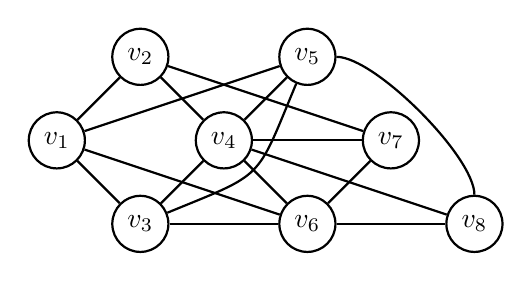
\begin{tikzpicture}[node distance={15mm}, thick, main/.style = {draw, circle}] {Graph}
            \node[main] (a) {$v_1$}; 
            \node[main] (b) [above right of=a] {$v_2$}; 
            \node[main] (c) [below right of=a] {$v_3$}; 
            \node[main] (d) [above right of=c] {$v_4$}; 
            \node[main] (e) [above right of=d] {$v_5$}; 
            \node[main] (f) [below right of=d] {$v_6$}; 
            \node[main] (g) [below right of=e] {$v_7$}; 
            \node[main] (h) [below right of=g] {$v_8$}; 
            \draw (a) -- (b); 
            \draw (a) -- (c); 
            \draw (a) -- (e); 
            \draw (b) -- (d); 
            \draw (c) -- (d); 
            \draw (e) -- (d); 
            \draw (e) to [out=247.5, in=22.5, looseness=1.5] (c); 
            \draw (f) -- (d); 
            \draw (g) -- (f); 
            \draw (g) -- (d); 
            \draw (f) -- (a); 
            \draw (g) -- (b);
            \draw (e) to [out=360, in=90, looseness=0.5] (h); 
            \draw (h) -- (d);
            \draw (h) -- (f);
            \draw (c) -- (f);
        \end{tikzpicture}
        \caption{The graph $G$}
        \label{fig:Graph}
     \end{subfigure}
     \hfill
     \begin{subfigure}{0.45\textwidth}
         \centering
         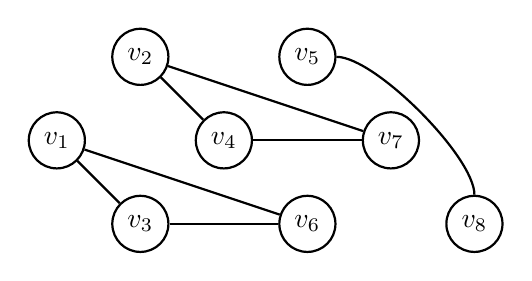
\begin{tikzpicture}[node distance={15mm}, thick, main/.style = {draw, circle}] {Graph}
            \node[main] (a) {$v_1$}; 
            \node[main] (b) [above right of=a] {$v_2$}; 
            \node[main] (c) [below right of=a] {$v_3$}; 
            \node[main] (d) [above right of=c] {$v_4$}; 
            \node[main] (e) [above right of=d] {$v_5$}; 
            \node[main] (f) [below right of=d] {$v_6$}; 
            \node[main] (g) [below right of=e] {$v_7$}; 
            \node[main] (h) [below right of=g] {$v_8$}; 
            \draw (a) -- (c); 
            \draw (f) -- (a); 
            \draw (c) -- (f);
            \draw (b) -- (d);
            \draw (g) -- (d); 
            \draw (g) -- (b);
            \draw (e) to [out=360, in=90, looseness=0.5] (h); 
        \end{tikzpicture}
        \caption{An optimal partition in $G$}
        \label{fig:Partition}
    \end{subfigure}
    \caption{An example for the MaxUtil problem where $k=3$.}
%    \label{}
\end{figure}

\subsection{The Hardness of the MaxUtil Problem}
The MaxUtil problem when $k=2$ is equivalent to the maximum matching problem, and thus it can be computed in polynomial time \cite{edmons1965paths}.
However, our problem becomes intractable when $k \geq 3$. 
%For the hardness proof we use the problem of partition into triangles, which was shown to be in $NP$-Complete \cite{di2004np}.
% Specifically, in this problem the goal is to decide whether the vertices of a graph $G$ can be partitioned into $q$ disjoint sets $V_1, V_2, . . . , V_q$, each containing exactly $3$ vertices, such that each of these $V_i$ is the node set of a triangle in $G$.
For the hardness proof, we define for each $k \in \mathbb{N}$ the $Cliques_k$ problem, which is as follows.
\begin{definition}[$Cliques_k$]
Given an undirected graph $G=(V,E)$, decide whether $V$ can be partitioned into disjoint cliques, such that each clique is composed of exactly $k$ vertices.
\end{definition}
Clearly, $Cliques_2$ can be decided in polynomial time by computing a maximum matching of the graph $G$, $M$, and testing whether $|M| = \frac{|V|}{2}$.
However, $Cliques_k$ becomes hard when $k\geq 3$.
\begin{lemma}
$Cliques_k$ is in $NP$-Complete for every $k\geq3$.
\end{lemma}
\begin{proof}
Clearly, $Cliques_k$ is in $NP$ for every $k$.
We use induction to show that any $Cliques_k$ is in $NP$-Hard for every $k\geq 3$.
$Cliques_3$ is known as the `partition into triangles' problem, which was shown to be in $NP$-Complete \cite{garey1979computers}.
Given that $Cliques_k$ is in $NP$-Hard we show that $Cliques_{k+1}$ is also in $NP$-Hard.
Given an instance of the $Cliques_k$ on a graph $G(V,E)$, we construct the following instance. We build a graph $G'(V',E')$, in which we add a set of nodes $\hat{V} = {\hat{v}_1, ..., \hat{v}_{\frac{|V|}{k}}}$, i.e., $V' = V \cup \hat{V}$. If $e \in E$ then $e \in E'$, and for every $v \in V, \hat{v} \in \hat{V}$ we add $(v,\hat{v})$ to $E'$.
%Clearly, $Cliques_\kappa(G) = Cliques_{\kappa+1}(G')$.
Clearly, $V$ can be partitioned into disjoint cliques with exactly $k$ vertices if and only if $V'$ can be partitioned into disjoint cliques with  exactly $k+1$ vertices.
\end{proof}


\begin{theorem}
The decision variant of the MaxUtil problem is in $NP$-Complete.
\end{theorem}
\begin{proof}
Clearly the problem is in $NP$, since if we are given a partition $P$, a limit $k$, and the value $\upsilon$, we can easily check that $\forall  S \in P$, $|S| \leq k$ and that $u(P) \geq \upsilon$ in polynomial time. For the hardness proof, we use the $Cliques_k$ problem. 
Given an instance of $Cliques_k$ on a graph $G(V,E)$, we use the same graph with the same $k$ and $\upsilon = |V|(k-1)$ as an instance to the MaxUtil problem. Clearly, $V$ can be partitioned into disjoint cliques with exactly $k$ vertices if and only if there exist a $k$-bounded partition $P$ such that $u(P) = \upsilon$.
\end{proof}

\subsection{Approximation of the MaxUtil Problem}
Since we showed that the MaxUtil problem is in $NP$-Complete, we now provide the Match and Merge (MnM) algorithm (Algorithm \ref{alg:MnM}), which is a polynomial-time approximation algorithm for any $k \geq 3$. 
%merge/union-match
The algorithm consists of $k-1$ rounds. Each round is composed of a matching phase followed by a merging phase.
Specifically, in round $l$ MnM computes a maximum matching, $M_l \subseteq E_l$, for $G_l$ (where $G_1 = G$). In the merging phase, MnM creates a graph $G_{l+1}$ that includes a unified node for each pair of matched nodes. $G_{l+1}$ also includes all unmatched nodes, along with their edges to the unified nodes (lines \ref{line:marge_edges_s}-\ref{line:marge_edges_e}).
Clearly, each node in $V_l$ is composed of up-to $l$ nodes from $V_1$.
Finally, MnM returns the $k$-bounded partition, $P$, of all the matched sets.
%
For example, given the graph $G_1$ in Figure \ref{fig:G_1} and $k=4$, the algorithm finds a maximum matching $M_1 = \{(v_1,v_2),(v_3,v_4)\}$ shown in Figure \ref{fig:M_1}.  It then creates the graph $G_2$, as shown in Figure \ref{fig:G_2}, and finds a maximum matching for it, $M_2 = \{(v_{3,4},v_5)\}$ shown in Figure \ref{fig:M_2}. It then creates the graph $G_3$, as shown in Figure \ref{fig:G_3}, and finds a maximum matching for it, $M_3=\{(v_{3,4,5}, v_6)\}$. 
Finally, MnM created the graph $G_4$, as shown in Figure \ref{fig:G_4}, and returns the $4$-bounded partition $P={\{v_1,v_2\},\{v_3,v_4,v_5,v_6\}}$.
We note that by the algorithm construction, a unified node $v_{i_1,...,i_l}$, is created by merging nodes $v_{i_1}$ and $v_{i_2}$, and then by merging $v_{i_1,i_2}$ and $v_{i_3}$, and so on.
 
\begin{algorithm}[ht]
    \caption{Match and Merge (MnM)}
    \label{alg:MnM}
    \SetAlgoLined
    \textbf{Input}:
    A graph $G(V,E)$ and a limit $k$\\
    \KwResult{A $k$-bounded partition $P$ of $V$.} 
    $G_1(V_1, E_1) \leftarrow G(V,E)$\\
    \For{$l\leftarrow1$ to $k-1$}{
        $M_l$ $\leftarrow$ maximum matching in $G_l$\\
        $G_{l+1}=(V_{l+1},E_{l+1}) \leftarrow$ an empty graph\\
        $V_{l+1} \leftarrow V_l$\\
        \For{\upshape every $(v_{i_1,...,i_l}, v_j) \in M_l$}{
            add vertex $v_{i_1,...,i_l,j}$ to $V_{l+1}$\\
            remove $v_{i_1,...,i_l}, v_j$ from $V_{l+1}$
        }
        \For{\upshape every $v_{i_1,...,i_{l+1}} \in V_{l+1}$}{\label{line:marge_edges_s}
            \For{\upshape every $v_q \in V_{l+1}$}{
                %\If {\upshape $(v_{i_1,...,i_{l+1}}, v_q) \in E_l$ }{
                \If {\upshape $(v_{i_1,...,i_l}, v_q) \in E_l$ or $(v_{i_{l+1}}, v_q) \in E_l$}{
                    add $(v_{i_1,...,i_{l+1}}, v_q)$ to $E_{l+1}$
                }
            }
        }\label{line:marge_edges_e}
    }
    
     $P \leftarrow$ an empty partition\\
     \For{\upshape every $v_{i_1,...,i_j} \in G_k$}{
         add the set $\{v_{i_1},...,v_{i_j}\}$ to $P$
     }
    % \For{\upshape every $v_i \in V_1$}{
    %     add the set $\{v_i\}$ to $P$
    % }
    % \For{$l \leftarrow 1$ to $k-1$}{
    %     \For{\upshape every $(v_{i_1,...,i_{l}}, v_j) \in M_l$}{
    %         add the set $\{v_{i_1},...,v_{i_l},v_j\}$ to $P$\\
    %         remove $\{v_{i_1,...,i_{l}}\}, \{v_j\}$ from $P$\\
    %     }
    % }
    \textbf{return} P
\end{algorithm}

\begin{figure}[ht]
    \centering
    \begin{subfigure}{.45\columnwidth}
        \centering
        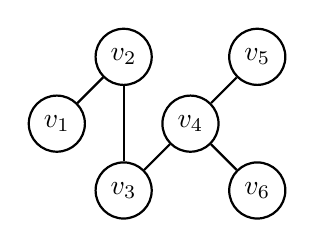
\begin{tikzpicture}[node distance={12mm}, thick, main/.style = {draw, circle}] {Graph}
        \node[main] (1) {$v_1$}; 
        \node[main] (2) [above right of=1] {$v_2$}; 
        \node[main] (3) [below right of=1] {$v_3$}; 
        \node[main] (4) [above right of=3] {$v_4$}; 
        \node[main] (5) [above right of=4] {$v_5$}; 
        \node[main] (6) [below right of=4] {$v_6$}; 
        \draw (1) -- (2); 
        \draw (3) -- (2); 
        \draw (3) -- (4); 
        \draw (4) -- (5); 
        \draw (4) -- (6); 
        \end{tikzpicture}
        \caption{The graph $G_1$}
        \label{fig:G_1}
    \end{subfigure}
    \begin{subfigure}{.45\columnwidth}
        \centering
        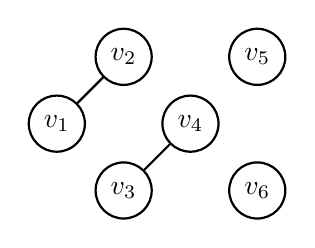
\begin{tikzpicture}[node distance={12mm}, thick, main/.style = {draw, circle}] {Graph}
        \node[main] (1) {$v_1$}; 
        \node[main] (2) [above right of=1] {$v_2$}; 
        \node[main] (3) [below right of=1] {$v_3$}; 
        \node[main] (4) [above right of=3] {$v_4$}; 
        \node[main] (5) [above right of=4] {$v_5$}; 
        \node[main] (6) [below right of=4] {$v_6$}; 
        \draw (1) -- (2); 
        \draw (3) -- (4); 
        \end{tikzpicture}
        \caption{The Matching $M_1$}
        \label{fig:M_1}
    \end{subfigure}
    \begin{subfigure}{.45\columnwidth}
        \centering
        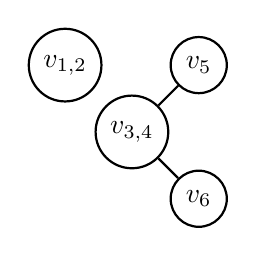
\begin{tikzpicture}[node distance={12mm}, thick, main/.style = {draw, circle}] {Graph}
        \node[main] (12) {$v_{1,2}$}; 
        \node[main] (34) [below right of=12] {$v_{3,4}$};  
        \node[main] (5) [above right of=34] {$v_5$}; 
        \node[main] (6) [below right of=34] {$v_6$}; 
        \draw (34) -- (5); 
        \draw (34) -- (6); 
        \end{tikzpicture}
        \caption{The graph $G_2$}
        \label{fig:G_2}
    \end{subfigure}
    \begin{subfigure}{.45\columnwidth}
        \centering
        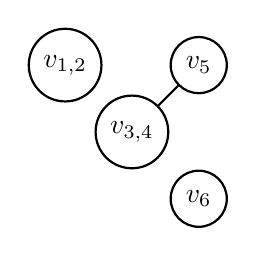
\begin{tikzpicture}[node distance={12mm}, thick, main/.style = {draw, circle}] {Graph}
        \node[main] (12) {$v_{1,2}$}; 
        \node[main] (34) [below right of=12] {$v_{3,4}$};  
        \node[main] (5) [above right of=34] {$v_5$}; 
        \node[main] (6) [below right of=34] {$v_6$}; 
        \draw (34) -- (5); 
        \end{tikzpicture}
        \caption{The Matching $M_2$}
        \label{fig:M_2}
    \end{subfigure}
    \begin{subfigure}{.45\columnwidth}
        \centering
        \begin{tikzpicture}[node distance={12mm}, thick, main/.style = {draw, circle}] {Graph}
        \node[main] (12) {$v_{1,2}$}; 
        \node[main] (345) [below right of=12] {$v_{3,4,5}$};  
        \node[main] (6) [below right of=34] {$v_6$}; 
        \draw (345) -- (6); 
        \end{tikzpicture}
        \caption{The graph $G_3$}
        \label{fig:G_3}
    \end{subfigure}
    \begin{subfigure}{.45\columnwidth}
        \centering
        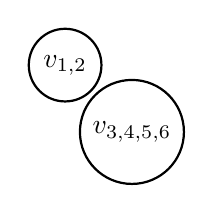
\begin{tikzpicture}[node distance={12mm}, thick, main/.style = {draw, circle}] {Graph}
        \node[main] (12) {$v_{1,2}$}; 
        \node[main] (3456) [below right of=12] {$v_{3,4,5,6}$};  
        \end{tikzpicture}
        \caption{The graph $G_4$}
        \label{fig:G_4}
    \end{subfigure}
    \caption{An example for Algorithm \ref{alg:MnM} where $k=4$.}
%    \label{}
\end{figure}



We now show that MnM provides an approximation ratio of $\frac{1}{k-1}$ for the MaxUtil problem. For that end, we first prove the following lemma related to the possible edges in every $G_l$, $l>1$.

\begin{lemma}
\label{lemma:5.5}
Given $\hat{v} = v_{i_1,...,i_l} \in V_l$, if there exist $v_i, v_j \in V_l$, $v_i\neq v_j$ such that $(v_i, v_{i_n}), (v_j, v_{i_m}) \in E$ for some $1 \leq n \leq m \leq l$, then $n = m$.
\end{lemma}

\begin{proof}
Observe that for every $v_i, v_j \in V_l$ where $l>1$, $(v_i,v_j) \notin E$, since $M_1$ is a maximum matching in $G_1$.
Assume by contradiction and without loss of generality that $n<m$. If $n=1$ and $m=2$, then the path $v_i \rightarrow v_{i_n} \rightarrow v_{i_m} \rightarrow v_j$ is an $M_1$-augmenting path in $G_1$ (\cite{edmons1965paths}), contrary to the fact that $M_1$ is a maximum matching in $G_1$. Therefore, $m\geq 3$. Consider the graph $G_2$, since $v_{i_m}, v_j \in V_2$, there exists an edge $(v_j, v_{i_m}) \in E$, contrary to our observation.







% We prove the lemma by induction on $l$.
% For $l=2$, the path $v_i \rightarrow v_{i_n} \rightarrow v_{i_m} \rightarrow v_j$ is an $M_1$-augmenting path in $G_1$ (\cite{edmons1965paths}), contrary to the fact that $M_1$ is a maximum matching in $G_1$. Therefore, the lemma is true for $l=2$.
% Assume by induction that the lemma is true for $l = \ell-1$, we show that the lemma is true also for $l = \ell$.
% Let $v_{i_\ell} \in V_{\ell-1}$ be the node we match to $\hat{v}$ in $M_{\ell-1}$.
% There is no $v_m \in V_{\ell-1}$ such that $(v_{i_\ell},v_m)\in E_{\ell-1}$. Otherwise, $v_{i_\ell} \rightarrow v_m$ is an augmenting path (\cite{edmons1965paths}) to $M_{\ell-1}$, contrary to the fact that $M_{\ell-1}$ is a maximum matching in $G_{\ell-1}$.
% The lemma is true for $l = \ell$.
% Therefore, Let $\hat{v} = v_{i_1,...,i_{l+1}}$, there are no two different nodes, $v_i, v_j$ s.t. $v_i, v_j, \hat{v}$ are in the same set in $Opt$ and $(v_i, v_{i_m}), (v_j, v_{i_n}) \in E_{\ell+1}$ for some $1 \leq m \neq n \leq l+1$.
\end{proof}





We now present a hypothetical procedure (Procedure \ref{alg:findMatch}) that is provided with a solution to the MaxUtil problem, which is a $k$-bounded partition $Opt$, a graph $G_l$ (as defined in Algorithm \ref{alg:MnM}), and a corresponding round index $l$. Without loss of generality, we assume that every set $S \in Opt$ is a connected component. %
%
%Let $O=\{v_o | \{v_o\} \in Opt\}$. That is, $|O|$ is the number of singletons in the partition $Opt$.
%
Let $O=\{v_o | \{v_o\} \in Opt$ and $v_o \in V_2\}$. That is, $|O|$ is the number of singletons in the partition $Opt$ that are also not matched in $M_1$. %
%
%be the group of all the nodes who are alone in the set in $Opt$.
We show that Procedure \ref{alg:findMatch} finds a matching, and we provide a lower bound on the size of this matching (the number of edges in it). %size of at least $\frac{|V_l'|-|O|}{k-1}$. 
We further show that MnM is guaranteed to perform at least as well as this procedure, which, as we show, results in an approximation ratio of $\frac{1}{k-1}$ for every $k\geq3$.


%Let $V_i'=\{v_i$ s.t. $v_i \in V_i\}$ be the group of all the unmatched nodes in $G_i$.

\begin{procedure1}[ht]
    \caption{Find matching}
    \label{alg:findMatch}
    \SetAlgoLined
    \textbf{Input}:\\
    A $k$-bounded partition $Opt$\\
    %A partition into triangles $T$\\
    A graph $G_l=(V_l,E_l)$\\
    %A round index $l$\\
    \KwResult{A matching in $G_l$} 
    $R_l \leftarrow$ an empty matching\\
    \For {\upshape each $v_i \in V_l$ such that $\{v_i\} \in Opt$}
        {remove $v_i$ from $V_l$}
    \For{\upshape each $v_q \in V_l$}{\label{line:loop_k>3}
        let $\hat{v}$ be a vertex $v_{i_1,...,i_l}$ such that $(v_q, \hat{v})\in E_l$ and for some $1\leq j\leq l$, $v_q$ and $v_{i_j}$ belong to the same set in $Opt$\\

        %\For{$m \leftarrow 1$ to $l$}{
            \For {\upshape each $v_n \neq v_q$}{ 
            \If {\upshape $(v_n, \hat{v}) \in E_l$ and exists $1\leq m\leq l$, s.t. $v_{i_m}$ and $v_n$ belong to the same set in $Opt$}{
                remove $v_n$ from $V_l$ }\label{line:remove_vn}
            }
        add $(v_q, \hat{v})$ to $R_l$\label{line:add_edge_k>3}
    }
    \textbf{return} $R_l$
\end{procedure1}



\begin{lemma}
\label{lem:Rl_size}
Procedure \ref{alg:findMatch} finds a matching, $R_l$, in the graph $G_l$, such that $|R_l| \geq (|V|-2|M_1|-\sum\limits_{i=2}^{l-1}|M_i|-|O|)/(k-1)$, where $l>1$.
\end{lemma}

\begin{proof}
We first show that Procedure \ref{alg:findMatch} finds a matching, $R_l$, in the graph $G_l$.
At each iteration of the loop in line \ref{line:loop_k>3}, we add an edge between a single node, $v_q$, and a unified node, $v_{i_1,...,i_l}$.
We consider each single node only once. Therefore, it is not possible to add a single node twice to $R_l$. Similarly, each time a unified node is added to $R_l$, every single node $v_n \neq v_q$ such that $v_{i_m}$ and $v_n$ belong to the same set in $Opt$, for some $1\leq m\leq l$, is removed from $V_l$. Therefore, a unified node is not added more than once. That is, $R_l$ is a matching in $G_l$.
% Now, assume by contradiction that we add a unified node, $\hat{v}$, more than once to $R_l$. Let $(v_i,\hat{v})$ be the edge that we add in the first time and let $(v_j,\hat{v})$ be the edge that we add in the second time. Note that $\hat{v} = v_{i_1,...,i_l}$ such that $v_i$ and $v_{i_n}$ belong to the same set in $Opt$.
% By definition, $(v_j, \hat{v}) \in E$ and $v_j$ is in the same set with some $v_{i_m}$ in $Opt$,
% then we have already deleted $v_j$ from $V$ in line \ref{line:remove_vn} in the iteration when we added $(v_i,\hat{v})$ to $R_l$. Therefore, a unified node is never added more than once to $R_l$. That is, $R_l$ is a matching in $G$.

We now show a lower bound on the size of $|R_l|$.
Let $V_l'=\{v_i | v_i \in V_l\}$, i.e., the set of all the single nodes in $G_l$.
In line \ref{line:remove_vn} we remove nodes only when $m=j$ (according to Lemma \ref{lemma:5.5}).
Given $\hat{v} = v_{i_1,...,i_l}$, there are at most $k-1$ different nodes, $v_{j_1},...,v_{j_k-1}$ that are in the same set with $\hat{v}$ in $Opt$. Therefore, in each iteration of the loop in line \ref{line:loop_k>3}, we remove at most $k-2$ single nodes in line \ref{line:remove_vn} while adding one edge to $R_l$ in line \ref{line:add_edge_k>3}.
Thus, at least $\frac{1}{k-1}$ of the single nodes in $v_l$ (who are not in $O$) are matched to a unified node. Therefore, $|R_l| \geq \frac{|V_l'|-|O|}{k-1}$.
Now, $|V_2'|=|V_1|-2|M_1|$. In addition, at each iteration $l>i>1$, $|M_i|$ single nodes are each added to a unified node. Therefore, $|V_l'|=|V_1|-2|M_1|-\sum\limits_{i=2}^{l-1}|M_i|$. 
In addition, $V=V_1$.
Overall, $|R_l| \geq (|V|-2|M_1|-\sum\limits_{i=2}^{l-1}|M_i|-|O|)/(k-1)$.
\end{proof}


\begin{theorem}
Algorithm \ref{alg:MnM} provides a solution for the MaxUtil problem with an approximation ratio of $\frac{1}{k-1}$ for every $k\geq 3$.
\end{theorem}

\begin{proof}
%The size of the optimal solution is at most the size of the $Cliques_k$ of all the node except the group $O$, that is, .
Let $P$ be the $k$-bounded partition returned by Algorithm \ref{alg:MnM}.
Clearly, $u(P) \geq 2\cdot\sum\limits_{i=1}^{k-1} |M_i|$.
For every $l\geq 1$, $M_l$ is a maximum matching and thus $|M_l| \geq |R_l|$. In addition, according to Lemma \ref{lem:Rl_size}, $|R_l| \geq \frac{|V|-2|M_1|-\sum\limits_{i=2}^{l-1} |M_i| - |O|}{k-1}$. 

%%%%%%%%%%%
Therefore, \[u(P) \geq 2\cdot\sum\limits_{i=1}^{k-1} |M_i| = 2|M_1| + 2\cdot \sum\limits_{i=2}^{k-1} |M_i|.\]
\[\sum\limits_{i=2}^{k-1} |M_i| = |M_2| + |M_3| + ... + |M_{k-1}| \geq\] \[|M_2| + |M_3| + ... + |M_{k-2}| + |R_{k-1}| \geq |M_2| + |M_3| + ... + |M_{k-2}| + \]\[\frac{|V| - |O| - 2|M_1| - |M_2| - ... - |M_{k-2}|}{k-1} =\] \[\frac{|V| - |O| - 2|M_1|}{k-1} + \frac{k-2}{k-1} \sum\limits_{i=2}^{k-2} |M_i| \geq\] \[ (1 + \frac{k-2}{k-1}) \cdot \frac{|V| - |O| - 2|M_1|}{k-1} + (\frac{k-2}{k-1})^2 \sum\limits_{i=2}^{k-3} |M_i| \geq ... \geq \]\[(1 + \frac{k-2}{k-1} + (\frac{k-2}{k-1})^2 + ... + (\frac{k-2}{k-1})^{k-3}) \cdot \frac{|V| - |O| - 2|M_1|}{k-1} + \]\[(\frac{k-2}{k-1})^{k-2} \sum\limits_{i=2}^{k-1-(k-2)} |M_i| =\]\[ \sum\limits_{i=0}^{k-3}\Big((\frac{k-2}{k-1})^i \cdot \frac{|V| - |O| - 2|M_1|}{k-1}\Big).\]

That is, \[u(P) \geq 2|M_1| + 2\cdot\sum\limits_{i=0}^{k-3}\Big((\frac{k-2}{k-1})^i \cdot \frac{|V| - |O| - 2|M_1|}{k-1}\Big) =\]
%
% Therefore, $M_{l+1} \geq M_l - \frac{M_l}{k-1} = \frac{k-2}{k-1} M_l$
%
% $\sum\limits_{i=2}^{k-1} |M_i|$ is greater than the sum of geometrical progression where $a_1 = |M_2| \geq \frac{|V_1|-|O|-2|M_1|}{k-1}$, $q=\frac{k-2}{k-1}$ and $n=k-2$. 
%
%Thus, $|P| \geq \sum\limits_{i=1}^{k-1} |M_i| = |M_1| + \sum\limits_{i=2}^{k-1} |M_i| \geq 
%
\[2|M_1| + 2\cdot\frac{|V|-|O|-2|M_1|}{k-1} \cdot \frac{(\frac{k-2}{k-1})^{(k-2)}-1}{\frac{k-2}{k-1} -1} =\] \[2|M_1| + 2(|V|-|O|-2|M_1|) \cdot \frac{(\frac{k-2}{k-1})^{(k-2)}-1}{(k-1)(\frac{k-2}{k-1} -1)} = \]\[ 2|M_1| - 2(|V|-|O|-2|M_1|)((\frac{k-2}{k-1})^{(k-2)}-1) = \]\[2(|V| - |O|)(1 - (\frac{k-2}{k-1})^{(k-2)}) - 2|M_1|(1 - 2 \cdot (\frac{k-2}{k-1})^{(k-2)}).\]

Next, we show that \[(1 - 2 \cdot (\frac{k-2}{k-1})^{(k-2)})\geq 0.\]
Let \[f(k) = (\frac{k-2}{k-1})^{k-2} \mbox{, for } k\geq 3.\] Thus \[f'(k) = \frac{(k-2)^{k-2}\big(ln(\frac{k-2}{k-1})(k-1) + 1\big)}{(k-1)^{k-1}}.\] 
Now, $\frac{(k-2)^{k-2}}{(k-1)^{k-1}} > 0$.
In addition, it is known that $ln(x) \leq x-1$~\cite{10.2307/3615890}, \\and thus \[ln(\frac{k-2}{k-1})(k-1) + 1 \leq -\frac{1}{k-1}(k-1) + 1 = 0\] Therefore, for all $k\geq3$, $f'(k) \leq 0$ and $f(k) \leq f(3) = \frac{1}{2}$.


Overall, since $|M_1| \leq \frac{|V|-|O|}{2}$, %and for $k\geq 3, (\frac{k-2}{k-1})^{(k-2)} \leq \frac{1}{2}$, 
\[u(P) \geq 2(|V| - |O|)(1 - (\frac{k-2}{k-1})^{(k-2)}) - 2\cdot\frac{|V|-|O|}{2}(1 - 2 \cdot (\frac{k-2}{k-1})^{(k-2)})\]\[ = %
%\frac{|V|}{2} - |O|(1 - (\frac{k-2}{k-1})^{(k-2)})\geq \frac{|V|}{2} - \frac{|O|}{2} 
|V|-|O|.\]
Now, since in $Opt$ there are at least $|O|$ singletons, then $u(Opt)$ is at most $(|V|-|O|)\cdot(k-1)$, which occurs when all nodes are partitioned into cliques of size $k$ (except those in $O$). That is, 
\[ u(P) \geq \frac{u(Opt)}{k-1}.\]
\end{proof}



Since finding a maximum matching in a graph can be computed in $O(|E|\sqrt{|V|})$, Algorithm \ref{alg:MnM} runs in $O(kn^{2.5})$ time.
Next, we show that our approximation ratio is tight. 

\begin{figure}
\centering
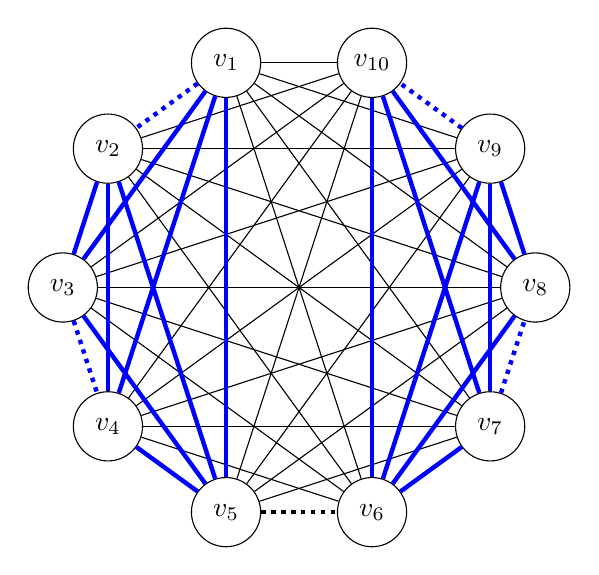
\begin{tikzpicture}
    \foreach \phi in {1,...,10}{
        \node[state] (v_\phi) at (72+ 360/10 * \phi:3cm){$v_{\phi}$};
    }
    \foreach \phi in {1,...,4}{
        \foreach \alpha in {6,...,10}{
            \draw (v_\phi) -- (v_\alpha);
        }
    }
    \foreach \alpha in {7,...,10}{
            \draw (v_5) -- (v_\alpha);
        }
    \foreach \i\j in {1/2,3/4,7/8,9/10}{
        \draw [blue, ultra thick, dotted](v_\i) -- (v_\j);
        }
    \foreach \i\j in {1/3,2/3,3/5,4/5}{
        \foreach \alpha in {\j,...,5}{
            \draw [blue, ultra thick] (v_\i) -- (v_\alpha);
        }
    }
    \foreach \i\j in {6/7,7/9,8/9}{
        \foreach \alpha in {\j,...,10}{
            \draw [blue, ultra thick] (v_\i) -- (v_\alpha);
        }
    }
    \draw [ultra thick, dotted](v_5) -- (v_6);
\end{tikzpicture}
\caption{An example of a graph in which $k=5$, and MnM achieves an approximation ratio of exactly $\frac{1}{4}$.}
\label{fig:complete_graph}
\end{figure}

\begin{theorem}
The approximation ratio of MnM for the MaxUtil problem is tight. 
\end{theorem}
\begin{proof}
Given $k>2$, consider a complete graph of size $2k$. In this case, MnM finds a perfect matching in $M_1$, and thus the partition $P$ returned by MnM contains $k$ groups of $2$ nodes. That is, $u(P) = 2k$. On the other hand, an optimal $k$-bounded partition $Opt$ consists of $2$ Cliques of size $k$, and thus $u(Opt) = 2k(k-1)$. That is, MnM provides an approximation of exactly $\frac{1}{k-1}$.
\end{proof}
Figure \ref{fig:complete_graph} presents a case where $k=5$, and $G$ is a complete graph with $10$ nodes. Here, $P=\{\{v_1,v_2\},\{v_3,v_4\},\{v_5,v_6\},\{v_7,v_8\},\{v_9,v_{10}\}\}$, as shown in the dotted lines, and thus $u(P) = 10$ . However, $Opt = \{\{v_1,v_2,v_3,v_4,v_5\}, \{v_6,v_7,v_8,v_9,v_{10}\}\}$, as shown in the blue lines, and $u(Opt) = 40$.


\subsection{Distributed Partition}
%TODO: correct this!!! All coallitions are a connected component!!!!
%Regarding the message of section 4.3, we attempt to show that when the agents are not fully coordinated, as assumed by our MnM algorithm, the social welfare for all agents may be reduced from 1/(k-1) to 1/k.

We now analyze a procedure that attempts to model the behavior of the agents when there is no central mechanism that determines the partition. Assume that the agents are split up arbitrarily but maximally, i.e., in a way that no two coalitions can joint together such that the social welfare will be higher. We call this procedure $Arbmax$. 
Without loss of generality, we assume that every set $S \in Arbmax$ is a connected component.
%We show that the uncoordinated procedure may result in an approximation ratio of only $\frac{1}{3}$; however, we show that a ratio of $\frac{1}{3}$ is guaranteed.
We show that $\frac{1}{k}$ is an upper bound on the approximation ratio that $Arbmax$ may guarantee.
\begin{theorem}
For any $k$, $Arbmax$ cannot guarantee an approximation ratio better than $\frac{1}{k}$
\end{theorem}
\begin{proof}
Given $k$, consider the following graph $G$. There are $k$ distinguished nodes, $v_1,\ldots,v_k$, with the edges  $(v_i,v_{i+1})\in E$ for $i=1,\ldots,k-1$. Each distinguished node $v_i$ has $k-1$ additional neighbors that are connected only to $v_i$, i.e., $v_i$ is the internal node of a star graph with $k-1$ leaves. Clearly, $Opt$ consists of $k$ coalitions, where each coalition consists of a star graph. Thus, $u(Opt)=2k(k-1)$. On the other hand, $Arbmax$ may partition the graph such that the distinguished nodes $v_1,\ldots,v_k$ are in the same coalition. Since there are no edges between two undistinguished nodes, the social welfare of this partition is $2(k-1)$. Therefore, $Arbmax$ cannot guarantee an approximation ratio better than $\frac{1}{k}$.
\end{proof}
Figure \ref{fig:Arbmax} presents a case where $k=5$, and $Arbmax$ may provide only a $\frac{1}{5}$ of the social welfare provided by an optimal solution. Here, $Arbmax$ may return the partition 
$P' = \{\{v_1, v_2, v_3, v_4, v_5\}, \{v_6\}, \{v_7\}, $ $ \{v_8\}, \{v_9\}, \{v_{10}\}, \{v_{11}\}, \{v_{12}\}, \{v_{13}\}, \{v_{14}\}, \{v_{15}\}, \{v_{16}\}, \{v_{17}\}, \{v_{18}\},$ \, $ \{v_{19}\}, \{v_{20}\}, \{v_{21}\}, \{v_{22}\}, \{v_{23}\}, \{v_{24}\}, \{v_{25}\}\}$ and thus $u(P') = 8$, while $Opt = \{\{v_1, v_6, v_7, v_8, v_9\}, \{v_2, v_{10}, v_{11}, v_{12}, v_{13}\}, \{v_3, v_{14}, v_{15}, $ \, $ v_{16}, v_{17}\}, \{v_4, v_{18}, v_{19}, v_{20}, v_{21}\}, \{v_5, v_{22}, v_{23}, v_{24}, v_{25}\}\}$ and therefore $u(Opt) = 40$.


\begin{figure}
\centering
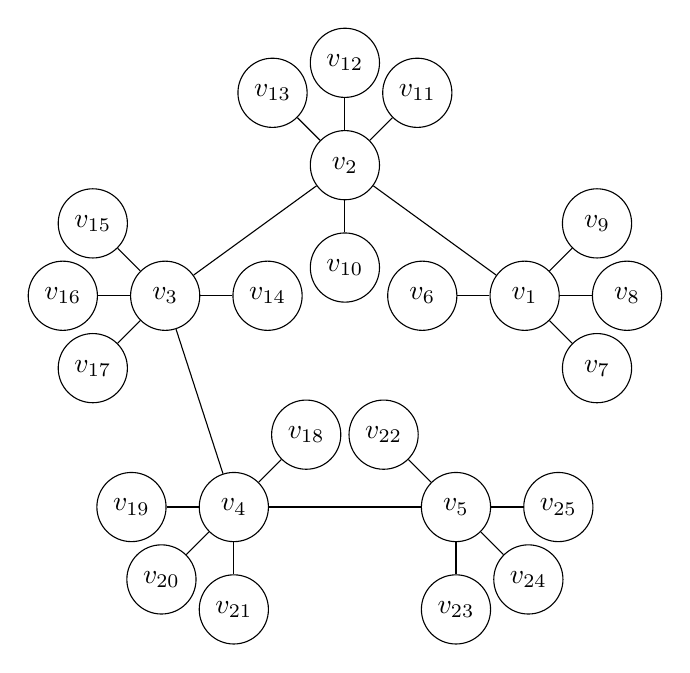
\begin{tikzpicture}[node distance={13mm}]
    \foreach \phi in {1,...,5}{
        \node[state] (\phi) at (-54 + 360/5 * \phi:2.4cm){$v_{\phi}$};
    }
    \node[state] (6) [left of=1] {$v_6$}; 
    \node[state] (7) [below right of=1] {$v_7$}; 
    \node[state] (8) [right of=1] {$v_8$}; 
    \node[state] (9) [above right of=1] {$v_9$}; 
    \node[state] (10) [below of=2] {$v_{10}$}; 
    \node[state] (11) [above right of=2] {$v_{11}$}; 
    \node[state] (12) [above of=2] {$v_{12}$}; 
    \node[state] (13) [above  left of=2] {$v_{13}$};
    \node[state] (14) [right of=3] {$v_{14}$}; 
    \node[state] (15) [above left of=3] {$v_{15}$}; 
    \node[state] (16) [left of=3] {$v_{16}$}; 
    \node[state] (17) [below left of=3] {$v_{17}$}; 
    \node[state] (18) [above right of=4] {$v_{18}$}; 
    \node[state] (19) [left of=4] {$v_{19}$}; 
    \node[state] (20) [below left of=4] {$v_{20}$}; 
    \node[state] (21) [below of=4] {$v_{21}$}; 
    \node[state] (22) [above left of=5] {$v_{22}$}; 
    \node[state] (23) [below of=5] {$v_{23}$}; 
    \node[state] (24) [below right of=5] {$v_{24}$}; 
    \node[state] (25) [right of=5] {$v_{25}$}; 
    \draw (1) -- (2);
    \draw (2) -- (3);
    \draw (3) -- (4);
    \draw (4) -- (5);
    \draw (1) -- (6);
    \draw (1) -- (7);
    \draw (1) -- (8);
    \draw (1) -- (9);
    \draw (2) -- (10);
    \draw (2) -- (11);
    \draw (2) -- (12);
    \draw (2) -- (13);
    \draw (3) -- (14);
    \draw (3) -- (15);
    \draw (3) -- (16);
    \draw (3) -- (17);
    \draw (4) -- (18);
    \draw (4) -- (19);
    \draw (4) -- (20);
    \draw (4) -- (21);
    \draw (5) -- (22);
    \draw (5) -- (23);
    \draw (5) -- (24);
    \draw (5) -- (25);
\end{tikzpicture}
\caption{A case where $k=5$, and $Arbmax$ may provide only a $\frac{1}{5}$ of the social welfare provided by an optimal solution.}
\label{fig:Arbmax}
\end{figure}
 
% Indeed, $Arbmax$ is guaranteed to provide an approximation ratio of $\frac{1}{k}$.
% \begin{theorem}
% $Arbmax$ provides an approximation with a ratio of $\frac{1}{k}$.
% \end{theorem}

% \begin{proof}
% Given a partition $P$, let $E_P = \{(u_i, u_j) \in E \mbox{: } \exists S \in Opt \mbox{ where } u_i,u_j \in S\}$. Note that $V_P$ is $2|E_P|$. We would like to show that $\frac{|E_{Arbmax}|}{{|E_{Opt}|}} \geq \frac{1}{k}$.

% %For that end we count how many more edges are in $E_{Opt}$ than in $E_{Arbmax}$ and show that $|E_{Arbmax} \setminus E_{Opt}| \geq \frac{1}{3} \cdot |E_{Opt} \setminus E_{Arbmax}|$. Therefore, we ignore edges that appear in both $E_{Opt}$ and $E_{Arbmax}$.
% %Consider the two sets of edges, $E_{Opt}$ and $E_{Arbmax}$, and 
% %Let $e = (u_i,u_j) \in E_{Opt} \setminus E_{Arbmax}$. Note that either $u_i$ or $u_j$ are not singletons in $Arbmax$; otherwise we can replace the singletons $\set{u_i}, \set{u_j}$ with the set $\set{u_i,u_j}$ in $Arbmax$, contrary to the assumption the $Arbmax$ is maximal. Without loss of generality, assume that $u_i$ is not a singleton in $Arbmax$. 

% To avoid double counting of the same edge, instead of counting edges, we give a weight of $\frac{1}{2}$ to each node at each edge.

% Let $e = (u_i,u_j) \in E_{Opt}$. Note that either $u_i$ or $u_j$ are not singletons in $Arbmax$; otherwise we can replace the singletons $\set{u_i}, \set{u_j}$ with the set $\set{u_i,u_j}$ in $Arbmax$, contrary to the assumption the $Arbmax$ is maximal. Without loss of generality, assume that $u_i$ is not a singleton in $Arbmax$. 
% There are two possible cases:
% \begin{itemize}
%     \item Case $1$ - $u_j$ is not a singleton in $Arbmax$. By definition,  every set in $Arbmax$ is a connected component. Therefore, each of the nodes $u_i, u_j$ adds at least $\frac{1}{2}$ to $V_{Arbmax}$. In $Opt$ each of the nodes $u_i, u_j$ can be connected to maximum $k-1$ others nodes. i.e., each, $u_i$ and $u_j$ adds at most $\frac{k-1}{2} \cdot 2$ to $V_{Opt}$. %$\frac{1}{2} \geq \frac{k-1}{3}$.
%     \item Case $2$ - $u_j$ is a singleton in $Arbmax$. The only possible option is that $u_i$ is in a full set, $S$, in $Arbmax$; i.e., $|S|=k$; otherwise we can replace the sets $\set{u_i}, S$ with the set $\set{u_i}\cup S$ in $Arbmax$, contrary to the assumption the $Arbmax$ is maximal.
%     Let $S = \{u_{i_1},..., u_{i_k}\}$. In $Opt$ each of the nodes $u_{i_1},...,u_{i_k}$ can be connected to maximum $k-1$ others nodes. i.e., each, $u_{i_1},...,u_{i_k}$ adds at most $K\frac{k-1}{2}$ to $V_{Opt}$. 
%     By definition, every set in $Arbmax$ is a connected component. Therefore, $V_S \geq k-1$. %$\frac{2}{6} \geq \frac{1}{3}$.
% \end{itemize}
% \end{proof}



\section{Stability}
When considering a stability concept $c$, we analyze the following two problems:
\begin{itemize}
    \item Existence: determine whether for any $(G,k)$ there exists a partition that satisfies $c$.
    %\item Verification: given $(G,k)$ and a partition, determine whether it satisfies $c$.
    \item Finding: given $(G,k)$, decide if there exists a partition that satisfies $c$ and if so, find such a partition.
\end{itemize}

\subsection{Nash Stable (NS)}

We begin our analysis with the (arguably) most basic stability concept, Nash stability. We show that for any $(G,k)$ a Nash stable $k$-bounded partition exists, and we present Algorithm \ref{alg:NS}, a polynomial time algorithm that finds such a partition. The algorithm begins with all agents in singletons and iteratively considers for each agent whether it may benefit from leaving her coalition and joining a coalition of size of at most $k-1$.
%\subsubsection{Existence  and Finding}

\begin{algorithm}[ht]
    \caption{Finding a Nash stable $k$-bounded partition}
    \label{alg:NS}
    \SetAlgoLined
    \textbf{Input}:
    A graph $G(V,E)$ and a limit $k$\\
    \KwResult{A $k$-bounded Nash Stable partition $P$ of $V$.} 
    $P \leftarrow \{\{v\}$ for every $v \in V\}$\\
    
    %\For{$i \leftarrow 1$ to $|E|$}{
    outerLoop:\\ \label{NS:outerLoop} 
        \For{$v \in V$}{
            \For{$S \in P$}{
                \If{$N(v,S \cup \{v\}) > u(v,P)$  AND $|S| \leq k-1$}{
                \label{NS:if}
                    $P \leftarrow P^{-S \cup \{v\}}$ \\
                    \textbf{goto} outerLoop
                }
            }
        }
        \textbf{return} P
\end{algorithm}

\begin{theorem}
There always exists a $k$-bounded Nash stable partition, and it can be found in polynomial time.
\end{theorem}

\begin{proof}
Consider Algorithm \ref{alg:NS}.
Clearly, when Algorithm \ref{alg:NS} terminates, the partition $P$ is a $k$-bounded Nash Stable partition.
We now show that Algorithm \ref{alg:NS} must always terminate, and it runs in polynomial time.
Returning to line \ref{NS:outerLoop} occurs only when the if statement in line \ref{NS:if} is true, which entails that $u(P)$ has increased. Since any increase in $u(P)$ must be by multiples of $2$, and since $u(P)$ is bounded by $2|E|$, the algorithm must terminate after at most $|E|$ iterations.
\end{proof}

% \subsubsection{Verification}
% Given the size limit, $k$, a graph, $G(V,E)$, and a $k$-bounded partition of its vertices, $P$, We can easily determine whether $P$ is $NS$. For every vertex $v \in V$ and for every coalition $S \in P$ such that $|S| < k$, we should only Verify that $u(v,P) \geq N(v,S\cup \{v\})$.



\subsection{Core}
The analysis of the core is more involved.
First, we show that for $k=3$ the core is never empty. We present Algorithm \ref{alg:core}, a polynomial time algorithm that finds a $3$-bounded partition $P$ in the core. The algorithm begins with all agents in singletons and iteratively considers for each $3$-bounded coalition whether it strongly blocks the current partition.

\begin{algorithm}[ht]
    \caption{Finding a $3$-bounded partition in the core}
    \label{alg:core}
    \SetAlgoLined
    \textbf{Input}:
    A graph $G(V,E)$\\
    \KwResult{A $3$-bounded partition $P$ of $V$ in the core.} 
    $P \leftarrow \{\{v\}$ for every $v \in V\}$\\
    $V' \leftarrow V$\\
    outerLoop:\\ 
    \label{core:outerLoop}
        \For{$S \subset V'$, such that $|S|=2$ OR $|S|=3$}{
            
            \If{$\forall v \in S, N(v ,S) > u(v,P)$}{
            \label{core:if}
                $P \leftarrow P^{-S}$ \\
                \If{$S$ is clique of size $3$}{
                    $V' \leftarrow V' \setminus S$\\ \label{alg:core:line:remove}
                }
                \textbf{goto} outerLoop
            }
        }
        \textbf{return} P
\end{algorithm}

\begin{theorem}
There always exists a $3$-bounded partition in the core, and it can be found in polynomial time.
\end{theorem}

\begin{proof}
Consider Algorithm \ref{alg:core}.
Note that for every $3$-bounded partition $P$, if $S \in P$ is a clique of size $3$ then every $v \in S$ cannot belong to any strongly blocking coalition. 
Therefore, Algorithm~\ref{alg:core} removes such vertices from $V'$ (in line~\ref{alg:core:line:remove}).
Clearly, if Algorithm \ref{alg:core} terminates, the $3$-bounded partition $P$ is in the core.
We now show that Algorithm \ref{alg:core} must always terminate, and it runs in polynomial time.
The algorithm initiates a new iteration (line  \ref{core:outerLoop}) whenever the if statement in line \ref{core:if} is true, which can happen when the blocking coalition $S$, is one of the following:
\begin{itemize}
    \item Only singletons (i.e., two or three singletons). Then, $u(P)$ increases by at least $2$.
    \item One agent from a coalition in which she has one neighbor, and two singleton agents. Then, $u(P)$ increases by at least $2$.
    \item Two agents, each from a coalition with a single neighbor, and one singleton agent. Then, $S$ must be a clique of size $3$, which increases $u(P)$ by $2$.
    \item Three agents, each from a coalition with a single neighbor. Then, $S$ must also be a clique of size $3$; however, $u(P)$ remains the same.
\end{itemize}
Overall, either $u(P)$ has increased by at least $2$ or $S$ is a clique of size $3$ and thus its vertices are removed from further consideration (in line~\ref{alg:core:line:remove}). %,and thus, until terminates, $P$ will never have any strongly blocking $3$-bounded coalition contains $v_i, v_j$ or $v_k$. 
Since $u(P)$ is bounded by $2|E|$ and the number of vertices is finite, the algorithm must terminate after at most $|E|+|V|/3$ iterations.
\end{proof}


For $k>3$ it is unclear whether the core can be empty, and how to find a partition in the core. Therefore, we now investigate additive and multiplicative approximations of the core, which are defined as follows. %, i.e., the ($\alpha$, $\beta$)-core.
%
\begin{definition}[Additive approximation]
A $k$-bounded coalition $S$ is said to \emph{$\epsilon_a$-strongly block} a $k$-bounded partition $P$ if it improves the utility of each of its members by more than an additive factor of $\epsilon_a$. That is, for every $v \in S$, $N(v,S) > u(v,P) + \epsilon_a$.
A $k$-bounded partition $P$ is in the \emph{$\epsilon_a$-core} if it does not have any $\epsilon_a$-strongly blocking $k$-bounded coalitions.
\end{definition}

The \emph{$\epsilon_m$-core}, which is the multiplicative approximation of the core is defined similarly. That is, a $k$-bounded coalition $S$ is said to \emph{$\epsilon_m$-strongly block} a $k$-bounded partition $P$ if for every $v \in S$, $N(v,S) > \epsilon_m \cdot u(v,P)$.

%\begin{definition}[Multiplicative Approximation]
% A $k$-bounded coalition $S$ is said to \emph{($\alpha$, $\beta$)-strongly block} a $k$-bounded partition $P$ if it improves the utility of each of its members by more than a multiplicative factor of $\alpha$ and an additive factor of $\beta$. i.e., for every $v \in S$, $N(v,S) > \alpha \cdot u(v,P) + \beta$.

% A $k$-bounded partition $P$ is in the \emph{($\alpha$, $\beta$)-core} if it does not have any ($\alpha$, $\beta$)-strongly blocking $k$-bounded coalitions.
% \end{definition}


We now show that for $k>3$ the $\epsilon_a$-core, for $\epsilon_a = \lfloor \frac{k}{2} \rfloor -1$, is never empty. We present Algorithm \ref{alg:Addcore}, a polynomial time algorithm that finds a $k$-bounded partition $P$ in the $\epsilon_a$-core. The algorithm begins with all agents in singletons and iteratively considers for each $k$-bounded coalition whether it $\epsilon_a$-strongly blocks the current partition.

\begin{algorithm}[ht]
    \caption{Finding a $k$-bounded partition in the $\epsilon_a$-core}
    \label{alg:Addcore}
    \SetAlgoLined
    \textbf{Input}:
    A graph $G(V,E)$\\
    A limit $k$\\
    An additive factor $\epsilon_a$\\
    \KwResult{A $k$-bounded partition $P$ of $V$ in the $\epsilon_a$-core.} 
    $P \leftarrow \{\{v\}$ for every $v \in V\}$\\
    $V' \leftarrow V$\\
    outerLoop:\\ 
    \label{Addcore:outerLoop}
        \For{$S \subset V'$, such that $1<|S|\leq k$}{
            \If{$\forall v \in S, N(v ,S) > u(v,P) + \epsilon_a$}{
            \label{Addcore:if}
                $P \leftarrow P^{-S}$ \\
                \If{$\forall v \in S, N(v ,S) \geq k-1-\epsilon_a$}{
                    $V' \leftarrow V' \setminus S$\\ \label{Addcore:line:remove}
                }
                \textbf{goto} outerLoop
            }
        }
        \textbf{return} P
\end{algorithm}

\begin{theorem}
For $\epsilon_a = \lfloor \frac{k}{2} \rfloor -1$, there always exists a $k$-bounded partition in the $\epsilon_a$-core, and it can be found in polynomial time.
\end{theorem}

\begin{proof}
Consider Algorithm \ref{alg:Addcore}.
Note that for every $k$-bounded partition $P$, and $S \in P$, if for every $v \in S$, $N(v ,S) \geq k-1-\epsilon_a$ then every $v \in S$ cannot belong to any $\epsilon_a$-strongly blocking $k$-bounded coalition.
Therefore, Algorithm~\ref{alg:Addcore} removes such vertices from $V'$ (in line~\ref{Addcore:line:remove}).
Clearly, if Algorithm \ref{alg:Addcore} terminates, the $k$-bounded partition $P$ is in the $\epsilon_a$-core.
We now show that for $\epsilon_a = \lfloor \frac{k}{2} \rfloor -1$, Algorithm \ref{alg:Addcore} must always terminate, and it runs in polynomial time.

First, we show that $u(P)$ never decreases.
The algorithm initiates a new iteration (line  \ref{Addcore:outerLoop}) whenever the if statement in line \ref{Addcore:if} is true. This can happen only if for every $v$ in the blocking coalition $S$, $u(v,P)$ is less than $k-1-\lfloor \frac{k}{2} \rfloor + 1$ (since $N(v ,S)$ is at most $k-1$). Therefore, $u(v,P) < k-\frac{k}{2}+\frac{1}{2} = \frac{k}{2}+\frac{1}{2}$.
Since $u(v,P)$ is a natural number, $u(v,P) \leq \frac{k}{2}-\frac{1}{2}$.
%which can happen when for every $v$ in the blocking coalition $S$, $u(v,P) \leq k-1-\lfloor \frac{k}{2} \rfloor$, i.e., $u(v,P) \leq k-1-\frac{k}{2}+\frac{1}{2} = \frac{k}{2}-\frac{1}{2}$. 
When $S$ breaks-off, the social welfare decreases by at most $2 \cdot \sum\limits_{v\in S} u(v,P)$, and increases by at least $\sum\limits_{v\in S} (u(v,P)+\lfloor \frac{k}{2} \rfloor)$.
Since $\sum\limits_{v\in S} (u(v,P)+\lfloor \frac{k}{2} \rfloor) \geq \sum\limits_{v\in S} (u(v,P)+ \frac{k}{2} - \frac{1}{2}) \geq \sum\limits_{v\in S} (u(v,P)+ u(v,P)) = 2 \cdot \sum\limits_{v\in S} u(v,P)$, then $u(P)$ never decreases.

Next, we show that if $u(P)$ remains the same, then vertices are removed from further consideration (in line~\ref{Addcore:line:remove}). Observe that $u(P)$ remaining the same entails that $2 \cdot \sum\limits_{v\in S} u(v,P) = \sum\limits_{v\in S} (u(v,P)+\lfloor \frac{k}{2} \rfloor)$.
That is, $\sum\limits_{v\in S} u(v,P) = \sum\limits_{v\in S} \lfloor \frac{k}{2} \rfloor$. Recall that for every $v \in S$, $u(v,P) \leq \frac{k}{2}-\frac{1}{2}$ and note that $\frac{k}{2}-\frac{1}{2} \leq \lfloor \frac{k}{2} \rfloor$. Therefore, if $u(P)$ remains the same, then for every $v \in S$, $u(v,P) = \frac{k}{2}-\frac{1}{2}$. %We note that this may happen only when $k$ is odd.
Now, since for every $v \in S$,  $N(v,S) > u(v,P) + \lfloor \frac{k}{2} \rfloor -1$ and $\epsilon_a \geq 1$, then $N(v,S) > \frac{k}{2} - \frac{1}{2} + \frac{k}{2} - \frac{1}{2} - 1 = k-2 \geq k-1-\epsilon_a$.
Therefore, all $v \in S$ are removed from further consideration. 

Overall, either $u(P)$ has increased by at least $2$ or vertices are removed from further consideration.
Since $u(P)$ is bounded by $2|E|$ and the number of vertices is finite, the algorithm must terminate after at most $|E|+\frac{|V|}{k}$ iterations.
\end{proof}


Next, we show that for $k>3$ the $\epsilon_m$-core, for $\epsilon_m = 2$, is never empty. We use Algorithm \ref{alg:Addcore}, with the following changes:
%
%The algorithm begins with all the agents in singletons and iteratively considers for each $k$-bounded coalition whether it $\epsilon_m$-strongly blocks the current partition. It terminates when the current partition has no $\epsilon_m$-strongly blocking coalitions.
%
%We use $MultAlgorithm$, that is Algorithm \ref{alg:Addcore} with the following changes:
\begin{itemize}
    \item The input of the algorithm is $\epsilon_m$ instead of $\epsilon_a$ (in line $3$).
    \item In line $8$, we check if for every $v$ in $S$, $N(v ,S) > \frac{u(v, P)}{\epsilon_m}$.
    \item In line $10$, we check if for every $v$ in $S$, $N(v,S) \geq \frac{k-1}{\epsilon_m}$.
\end{itemize}
We show that this algorithm finds a $k$-bounded partition $P$ in the $\epsilon_m$-core in polynomial time.

\begin{theorem}
For $\epsilon_m = 2$, there always exists a $k$-bounded partition in the $\epsilon_m$-core, and it can be found in polynomial time.
\end{theorem}

\begin{proof}
%Consider $MultAlgorithm$.
Clearly, if the algorithm terminates, the $k$-bounded partition $P$ is in the $\epsilon_m$-core.
%We now show that for $\epsilon_m = 2$, the algorithm must always terminate, and it runs in polynomial time.
We show that $u(P)$ always increases.
The algorithm initiates a new iteration whenever $\forall v \in S, N(v ,S) > \frac{u(v, P)}{\epsilon_m}$, which can happen only if $S$ breaks-off.
When $S$ breaks-off, the social welfare decreases by at most $2 \cdot \sum\limits_{v\in S} u(v,P)$, and increases by at least $\sum\limits_{v\in S} (2 \cdot u(v,P)+1)$.
Since $\sum\limits_{v\in S} (2 \cdot u(v,P)+1) > 2 \cdot \sum\limits_{v\in S} u(v,P)$, then $u(P)$ always increases.
%Since $u(P)$ is bounded by $2|E|$, the algorithm must terminate after at most $|E|$ iterations.
\end{proof}


Finally, we show in simulation that a simple heuristic always finds a partition that is in the core.
Our heuristic function works as follows:
\begin{enumerate}
    \item Start with a $k$-bounded partition $P$, where all the agents are singletons.
    \item Iterate randomly over all the $k$-bounded coalitions until a coalition $S$ is found, which strongly blocks the partition $P$.
    \item Update $P$ to be $P^{-S}$, and return to step $(2)$.
\end{enumerate}
The heuristic terminates when either there is no strongly blocking coalition for the partition $P$ (i.e., $P$ is in the core), or when in $100$ consecutive iterations all of the partitions have already been seen. In the later case, we restart the heuristic.

We test our heuristic function for $k=5$ over more than $100$ million random graphs of different types: 
\begin{itemize}
\item Random graphs of size $30$ with probability of $0.5$ for rewiring each edge.
\item Random trees of size $30$.
\item Random connected Watts–Strogatz small-world graphs of size $30$, where each node is joined with its $5$ nearest neighbors in a ring topology and with a probability of $0.5$ for rewiring each edge.
\end{itemize}
Our heuristic always found a $k$-bounded partition that is in the core. Moreover, we had to restart the heuristic in only $33$ instances, and then a $k$-bounded partition in the core was found.

\subsection{Strict Core (SC)}
%\subsubsection{Existence}
We first show that for every size limit, $k$, there is at least one graph where there is no $k$-bounded partition in the strict core.
Indeed, given a size limit $k$, we build the graph $G(V,E)$, which is a clique of size $k+1$. For every partition $P$ of $V$, let $S$ be a coalition in $P$ such that $|S| < k$. Now, any set of agents of size $k$ that also contains some $v \in S$ is a weakly blocking $k$-bounded coalition for $P$. 
%
% \subsubsection{Verification}
% \label{sec: SC verification}
% Given the size limit, $k$, a graph, $G(V,E)$, and a $k$-bounded partition of its vertices, $P$, We can easily determine whether $P$ is in the $SC$ or not. There are at most $|V+1|^k k$-bounded coalitions of $V$. For every such coalition $S$, we should only Verify that $S$ is not a weakly blocking $k$-bounded coalition for $P$.
Furthermore, even verifying the existence of the strict core is a hard problem.

\begin{definition}[$SC$ existence problem]
Given a coalition size limit $k$ and a graph $G$, decide whether a $k$-bounded partition exists that is in the strict core.
\end{definition}
\begin{theorem}
The $SC$ existence problem is in $NP$-hard.
\end{theorem}

\begin{proof}
%Base on section \ref{sec: SC verification}, the finding $SC$ problem is in $NP$. 
We use a reduction from $Cliques_k$ for the hardness proof. Given an instance of the $Cliques_k$ on a graph $G(V,E)$, we construct the following instance. We build a graph $G'(V',E')$ such that $V'$ contains all the nodes from $V$. In addition, for every $v_x \in V$ we add the nodes $\hat{v}_x$ and $v_x^1,\ldots,v_x^{k-1}$ to $V'$. Now, $E'$ contains all the edges of $E$, and for every $v_x \in V$ and $1 \leq i \leq k-1$ we add $(v_x,v_x^i), (v_x^i, \hat{v}_x)$ to $E'$. Finally, for every $v_x \in V$ and $1 \leq i,j \leq k-1$, $i \neq j$ we add $(v_x^i, v_x^j)$ to $E'$. 
Figure \ref{fig:findSC} shows this construction for a specific $v_x$ when $k=4$.
We first show that if $G$ cannot be partitioned into disjoint cliques of size $k$, then the strict core is empty. Indeed, assume that $G$ cannot be partitioned into disjoint cliques of size $k$, and let $P$ be a $k$-bounded partition of $V'$. Then, there is at least one vertex $v_x \in V$ that belongs to a coalition $S\in P$, such that either:
\begin{enumerate}
    \item $N(v_x,S) < k-1$, or
    \item $v_x^i \in S$ for some $i$ between $1$ and $k-1$.
\end{enumerate}
In case $1$, the coalition $\{v_x, v_x^1, \ldots, v_x^{k-1}\}$ is a weakly blocking $k$-bounded coalition. In case $2$, the coalition $\{\hat{v}_x, v_x^1, \ldots, v_x^{k-1}\}$ is a weakly blocking $k$-bounded coalition.
Therefore, if the strict core is not empty, then $G$ can be partitioned into disjoint cliques of size $k$.

We now show that if $G$ can be partitioned into disjoint cliques of size $k$, then the strict core is not empty. Clearly, in this case $G'$ can be partitioned into disjoint cliques of size $k$, and this partition is in the strict core. Therefore, if the strict core is empty, then $G$ cannot be partitioned into disjoint cliques of size $k$.
\end{proof}

\begin{figure}
\centering
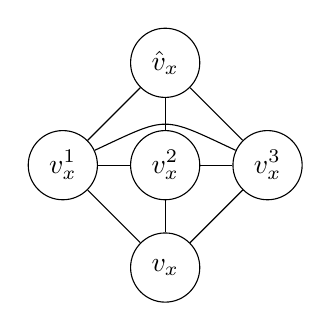
\begin{tikzpicture}[node distance={13mm}]
    \node[state] (1) {$v_x^1$}; 
    \node[state] (2) [right of=1] {$v_x^2$}; 
    \node[state] (3) [right of=2] {$v_x^3$}; 
    \node[state] (4) [above of=2] {$\hat{v}_x$}; 
    \node[state] (5) [below of=2] {$v_x$}; 
    
    \draw (1) -- (2);
    \draw (1) to [out=25, in=155, looseness=1.5] (3);
    \draw (2) -- (3);
    \draw (4) -- (1);
    \draw (4) -- (2);
    \draw (4) -- (3);
    \draw (5) -- (1);
    \draw (5) -- (2);
    \draw (5) -- (3);
    
\end{tikzpicture}
\caption{The reduction construction for a specific $v_x$ when $k=4$.}
\label{fig:findSC}
\end{figure}

\subsection{Contractual Strict Core (CSC)}
We show that the CSC is never empty. Indeed, given any $(G,k)$, the following algorithm finds a $k$-bounded partition in the CSC:
\begin{enumerate}
    \item Start with a $k$-bounded partition $P$, where all the agents are singletons.
    \item Iterate over all the coalitions in $P$ until two coalitions, $S_1, S_2$, are found, such that $|S_1|+|S_2| \leq k$ and $u(P) < u(P^{-S_1 \cup S_2})$.
    \item Update $P$ to be $P^{-S_1 \cup S_2}$, and return to step $(2)$.
\end{enumerate}
The algorithm terminates when step $2$ does not find two coalitions that meet the required conditions.

 \begin{theorem}
There always exists a $k$-bounded partition in the CSC, and it can be found in polynomial time.
\end{theorem}

\begin{proof}
At each iteration, the number of the coalitions in $P$ decreases and thus the algorithm must terminate after at most $k-1$ iterations.
Consider the $k$-bounded partition $P$ when the algorithm terminates. Clearly, there are no two coalitions in $P$ that can benefit from breaking off and joining together.
In addition, observe that every coalition $S \in P$ is a connected component. Thus, no coalition $S' \subsetneq S$ can break-off without decreasing the utility of at least one agent from $S\setminus S'$. 
Therefore, $P$ is in the CSC.   
\end{proof}

\section{Conclusions and Future Work}
In this paper, we initiate the study of ASHGs with a bounded coalition size. We provide MnM, an approximation algorithm for maximizing the utilitarian social welfare and study the computational aspects of Nash stability, the core, the SC, and the CSC. 
% move to conclusions
We note that MnM can be improved such that it finds a partition that is in the CSC while maintaining its approximation ratio. This is done by running MnM and iteratively joining together any two coalitions that improve the social welfare (without violating the size constraint).
%the partition is maximal, that is, no two groups can join together and add additional edges. %This will result in %think what will the lower bound be now.
%This can be achieved by first running MnM, and then adding back all the edges between any two unified nodes, as long as they may be merged together without violating the size capacity $k$. Multiple edges between two unified nodes, may either be simplified to a single edge, or may be associated with a weight proportionate to the number of edges. 
%Now, MnM can continue the process of matching and merging for up to $\frac{k}{2}$ additional rounds,
%but in the merging process it also adds the edges between two previously unified nodes, as long as they may be merged together without violating the size capacity $k$.

There are several interesting directions for future work. 
Since we show that the MaxUtil problem cannot be computed in polynomial time (unless $P=NP$), it will be interesting to investigate some variants. For example, the problem of finding a $k$-bounded partition such that each agent will be matched with at least one friend in its coalition.
%
%Another interesting research direction is to investigate strategic behavior of the agents when reporting their value from other agents.
%the strategic aspects of the problem. That is, treating the passengers as strategic agents who don't necessarily accept their assigned vehicle and may attempt to join a different vehicle, if it is more valuable for them.
%We will investigate the existence and the complexity of calculation of partitions that are swap stable, envy-free, find which partitions are in the core, which are pareto-optimal, etc. \cite{AZIZ2013316}
Another interesting research direction is to incorporate skills in our model, motivated by coalitional skill games \cite{bachrach2008coalitional}. That is, each agent has a set of skills, and each coalition is required to have at least one agent that acquires each of the skills.
%setting also with respect to the differences between drivers and passengers, i.e., some users may only be passengers, and it is not possible to group together only passengers (without a driver).

%NOT UPDATED:
%In this paper we argued that one way to promote ridesharing is by attempting to maximize the number of friendships in vehicles. For the that end we introduced the social aware assignment problem. In the social aware assignment problem there is a maximum fixed number of passengers in each vehicle, denoted by $k$, and the goal is to assign passengers such that the number of friendship relations is maximized. We showed that the  problem is trivial for the case of $k=2$, as it can be solved by a matching algorithm. However, we showed that the problem becomes computationally hard for any $k>2$. We therefore provided an efficient algorithm with an approximation ratio of $\frac{1}{k-1}$ and showed that this bound is tight. In addition, we analyzed the distributed case of this problem, in which the passengers split-up arbitrary but maximally, and showed that this procedure achieves an approximation ratio of, at most, $\frac{1}{k}$.
%
%In this paper we have discussed a case where the capacity of each vehicle is limited and identical. However, in practice, there are vehicles of various types and sizes. Therefore, in future work we will examine a case where there are vehicles with different capacities. It will be interesting to see how this will affect the behavior and approximation quality of MnM, and whether we can develop an algorithm more suitable to this problem.



%strategy proof - each user reports her friends, we want it to be honest.
%non-simple (i.e., the edges are weighted, possibly also negative and non-symmetric)



%lower bound for improved MnM (other than k=3)
%stability
%different sizes of vehicles



%%%%%%%%%%%%%%%%%%%%%%%%%%%%%%%%%%%%%%%%%%%%%%% other future work directions

%show that our method is stable. That is, no set of coalitions are (strictly?) better off when deviating.
%individual rational, trivial with no negative edges.
%individual stable, (no single user joins a different coalition and gains strictly more without harming new coalition). No negatives, whoever wants to may join (as long as there is room). so similar to Nash stable.
%Nash stable (no single user joins a different coalition and gains strictly more), negative example: triangles (can we improve until it becomes stable?). Social welfare increases each time and therefore it will always end.
%core (no group with everyone benefiting from deviating)
%strict core (no group with at least one benefiting from deviating)
%Pareto optimal: No, because for triangle problem, we must find the triangles. Therefore, according to page 319 in paper below, we are not in strict core.


%show that worst case of "random" without improvements is 1/3. (inner triangle example that gives 1/3).




%directed graph
%weights
%higher k (for 4, we can do three times, in second round prioritize the couples).
%negative (1,0,-1)
% Computing desirable partitions in additively separable hedonic games https://www.sciencedirect.com/science/article/pii/S000437021200118X/pdf?md5=a194e4bc669a23a85b15a8d7e1e929bd&pid=1-s2.0-S000437021200118X-main.pdf
%look at the proof used for showing that matching 3D is NP-Hard.

\bibliographystyle{ACM-Reference-Format} 
\bibliography{bibfile}

\end{document}
\endinput




% For clarity, we begin by providing Algorithm \ref{alg:approximation3}, which is an approximation algorithm for the case of $k=3$. In the following section, we generalize this algorithm to any $k\geq 3$.

% Algorithm \ref{alg:approximation3} works as follows. It first computes a maximum matching, $M \subseteq E$, for the given graph $G$. It then creates a graph $G'$ that includes a merged node for each pair of matched nodes. $G'$ also includes all unmatched nodes, along with their edges to the merged nodes
% (lines \ref{line:edges_to_E'1}-\ref{line:edges_to_E'2}).
% Finally, it computes a maximum matching for $G'$ and returns a partition, $P$, in which any two nodes that were merged are together, along with any node matched with them.
% %of all the matched sets.
% For example, given the graph $G$ in Figure \ref{fig:G}, the algorithm finds the maximum matching $M = \{(v_1,v_2),(v_3,v_4)\}$, which is shown in Figure \ref{fig:M}. The algorithm then creates the graph $G'$ (Figure \ref{fig:G'}), and finds the maximum matching $M'=\{(v_{3,4}, v_5)\}$. The algorithm thus returns the partition $P={\{v_1,v_2\},\{v_3,v_4,v_5\},\{v_6\}}$ (Figure \ref{fig:P}).

 % \begin{enumerate}
    %     \item Given a graph $G=(V,E)$, find a maximum matching, $M$, in $G$. %\cite{duan2014linear}.
    %     \item Create an undirected graph $G' = (V',E')$ such that $\forall (v_i, v_j) \in M$. Create a node $v_{i,j} \in V'$ and $\forall v_i \in V$, $v_i \in V'$ if there is no $v_j \in V$ such that $(v_i,v_j) \in M$. 
    %     In addition, $\forall v_{i,j}, v_k \in V'$, $(v_{i,j}, v_k) \in E'$ if $(v_i,v_k) \in E$ or $(v_j,v_k) \in E$ %$\forall v_i,v_j \in V', (v_i,_j) \in E'$ if $ (v_i,v_j) \in E$ and 
    %     \item Find a maximum matching in $G'$.
    % \end{enumerate}
    


    % \begin{algorithm}[ht]

    %     \caption{Approximation}
    %     \label{alg:approximation3}
    %     \SetAlgoLined
    %     \textbf{Input}:
    %     A graph $G=(V,E)$\\
    %     \KwResult{A partition $P$ of $G$ where $k=3$.} 
    %     M $\leftarrow$ maximum matching in $G$\\
    %     $G'=(V',E') \leftarrow$ an empty graph\\
    %     $V' \leftarrow V$\\
    %     \For{\upshape every $(v_i, v_j) \in M$}{
    %         Add vertex $v_{i,j}$ to $V'$\\
    %         remove $v_i, v_j$ from $V'$
    %     }
        
    %     \For{\upshape every $(v_i, v_j) \in M$}{\label{line:edges_to_E'1}
    %         \For{\upshape every $v_k \in V'$}{
    %             \If {\upshape $(v_i, v_k) \in E$ OR $(v_j, v_k) \in E$}{
    %                 Add edge $(v_{i,j}, v_k)$ to $E'$
    %             }
    %         }
    %     }\label{line:edges_to_E'2}
    %     $M' \leftarrow$ maximum matching in $G'$\\
    %     $P \leftarrow$ an empty partition\\
    %     \For{\upshape every $v_i \in V$}{
    %         add the set $\{v_i\}$ to $P$
    %     }
    %     \For{\upshape every $(v_i, v_j) \in M$}{
    %         add the set $\{v_i,v_j\}$ to $P$\\
    %         remove $\{v_i\}, \{v_j\}$ from $P$\\
    %     }
    %     \For{\upshape every $(v_{i,j}, v_k) \in M'$}{
    %         add the set $\{v_i,v_j,v_k\}$ to $P$\\
    %         remove $\{v_{i,j}\}, \{v_k\}$ from $P$\\
    %     }
    %     \textbf{return} P
    % \end{algorithm}

    % \begin{figure}[ht]
    %     \centering
    %     \begin{minipage}{.45\columnwidth}
    %         \centering
    %         \begin{tikzpicture}[node distance={12mm}, thick, main/.style = {draw, circle}] {Graph}
    %         \node[main] (1) {$v_1$}; 
    %         \node[main] (2) [above right of=1] {$v_2$}; 
    %         \node[main] (3) [below right of=1] {$v_3$}; 
    %         \node[main] (4) [above right of=3] {$v_4$}; 
    %         \node[main] (5) [above right of=4] {$v_5$}; 
    %         \node[main] (6) [below right of=4] {$v_6$}; 
    %         \draw (1) -- (2); 
    %         \draw (3) -- (2); 
    %         \draw (3) -- (4); 
    %         \draw (4) -- (5); 
    %         \draw (4) -- (6); 
    %         \end{tikzpicture}
    %         \caption{The graph G}
    %         \label{fig:G}
    %     \end{minipage}
    %     \begin{minipage}{.45\columnwidth}
    %         \centering
    %         \begin{tikzpicture}[node distance={12mm}, thick, main/.style = {draw, circle}] {Graph}
    %         \node[main] (1) {$v_1$}; 
    %         \node[main] (2) [above right of=1] {$v_2$}; 
    %         \node[main] (3) [below right of=1] {$v_3$}; 
    %         \node[main] (4) [above right of=3] {$v_4$}; 
    %         \node[main] (5) [above right of=4] {$v_5$}; 
    %         \node[main] (6) [below right of=4] {$v_6$}; 
    %         \draw (1) -- (2); 
    %         \draw (3) -- (4); 
    %         \end{tikzpicture}
    %         \caption{The Matching M}
    %         \label{fig:M}
    %     \end{minipage}
    %     \begin{minipage}{.45\columnwidth}
    %         \centering
    %         \begin{tikzpicture}[node distance={12mm}, thick, main/.style = {draw, circle}] {Graph}
    %         \node[main] (12) {$v_{1,2}$}; 
    %         \node[main] (34) [below right of=12] {$v_{3,4}$};  
    %         \node[main] (5) [above right of=34] {$v_5$}; 
    %         \node[main] (6) [below right of=34] {$v_6$}; 
    %         \draw (34) -- (5); 
    %         \draw (34) -- (6); 
    %         \end{tikzpicture}
    %         \caption{The graph G'}
    %         \label{fig:G'}
    %     \end{minipage}
    %     \begin{minipage}{.45\columnwidth}
    %         \centering
    %         \begin{tikzpicture}[node distance={12mm}, thick, main/.style = {draw, circle}] {Graph}
    %         \node[main] (1) {$v_1$}; 
    %         \node[main] (2) [above right of=1] {$v_2$}; 
    %         \node[main] (3) [below right of=1] {$v_3$}; 
    %         \node[main] (4) [above right of=3] {$v_4$}; 
    %         \node[main] (5) [above right of=4] {$v_5$}; 
    %         \node[main] (6) [below right of=4] {$v_6$};
    %         \draw (1) -- (2); 
    %         \draw (3) -- (4);
    %         \draw (4) -- (5);
    %         \end{tikzpicture}
    %         \caption{The partition P}
    %         \label{fig:P}
    %     \end{minipage}
    % \end{figure}
    
% We first present a theoretical procedure that, given an optimal partition $Opt$ and $G'$, finds a matching with a size of at least $\frac{|V|-2|M|-|O|}{2}$. Where $O=\{v_o$ s.t. $\{v_o\} \in Opt\}$. We will show that Algorithm \ref{alg:approximation3} is guaranteed to perform at least as well as this procedure, which results in an approximation ratio of $0.5$ for $k=3$.
% Without loss of generality, we assume that every set $S \in Opt$ is a connected component. 

% \begin{algorithm}[ht]
%     \caption{Find_matching}
%     \label{alg:findMatch}
%     \SetAlgoLined
%     \textbf{Input}:\\
%     The optimal partition $Opt$\\
%     %A partition into triangles $T$\\
%     A graph $G'=(V',E')$\\
%     \KwResult{A matching in $G'$} 
%     $R \leftarrow$ an empty matching\\
%     \For {\upshape each $v_i$ such that $\{v_i\} \in Opt$}
%         {remove $v_i$ from $V'$}
%     \For{\upshape each $v_i \in V'$}{\label{line:loop}
%         let $\hat{v}$ be $v_{j,k}$ or $v_{k,j}$ such that $v_i$ and $v_j$ belong to the same set in $Opt$ and $(v_i, \hat{v})\in E'$\\
%             %\If{\upshape $\{v_i, v_j, v_k\} \notin Opt$}{
%                 \For {\upshape each $v_l \neq v_i$ such that $v_j, v_l$ belong to the same set in $Opt$}{
%                     remove $v_l$ from $V'$ }\label{line:remove_vlvj}
%                 \For {\upshape each $v_l \neq v_i$ such that $v_k, v_l$ belong to the same set in $Opt$ and $(v_l,\hat{v})\in E'$}{
%                 remove $v_l$ from $V'$ }\label{line:remove_vlvk}
%             %}
%         add $(v_i, \hat{v})$ to $R$\label{line:add_edge}
%     }
%     \textbf{return} $R$
% \end{algorithm}

% %We want to show that even in this situation, when $k=3$, Then, algorithm \ref{alg:approximation} provides a solution for the social aware assignment problem with an approximation ratio of $0.5$.

% \begin{lemma}
% Procedure \ref{alg:findMatch} finds a matching, $R$, in the graph $G'$.
% \end{lemma}

% \begin{proof}
% At each iteration of the loop in line \ref{line:loop}, we add an edge between a single node and a unified node.
% We go over each single node only once. Therefore, it is not possible to add a single node twice to $R$.
% Now, assume by contradiction that we add a unified node, $\hat{v}$, more than once to $R$. Let $(v_i,\hat{v})$ be the edge that we add in the first time and let $(v_l,\hat{v})$ be the edge that we add in the second time. Note that $\hat{v} = v_{j,k}$ or $v_{k,j}$ such that $v_i$ and $v_j$ belong to the same set in $Opt$.
% By definition, $(v_l, \hat{v}) \in E'$ and $v_l$ is in the same set with $v_j$ or $v_k$ in $Opt$.
% If $v_l$ and $v_j$ are in the same set in $Opt$, then we have already deleted $v_l$ from $V'$ in line \ref{line:remove_vlvj} in the iteration when we added $(v_i,\hat{v})$ to $R$. Otherwise, since $v_l$ and $v_k$ are in the same set in $Opt$ and $(v_l, \hat{v}) \in E'$, we have already deleted $v_l$ from $V'$ in line \ref{line:remove_vlvk} in the iteration when we added $(v_i,\hat{v})$ to $R$. Therefore, a unified node is never added more than once to $R$. That is, $R$ is a matching in $G'$.
% \end{proof}

% \begin{lemma}
% Given the optimal partition $Opt$, procedure \ref{alg:findMatch} finds a matching, $R$, in the graph $G'$ such that $|R| \geq \frac{|V|-2|M|-|O|}{2}$.
% \end{lemma}

% \begin{proof}

% There are $|M|$ unified nodes in $V'$, where each node is composed of two nodes from $V$.  Therefore, there are exactly $|V| -2|M|$ single nodes in $V'$. 
% Suppose we delete some $v_l$ in line \ref{line:remove_vlvj}. By definition $(v_k, v_l) \in E$. The path $v_i \rightarrow v_j \rightarrow v_k \rightarrow v_l$ is an augmenting path (\cite{edmons1965paths}) to $M$, contrary to the fact that $M$ is a maximum matching in $G$. Therefore, we never delete any node in line \ref{line:remove_vlvk}.
% When $k=3$, there is only one possible node $v_l$ such that ${v_i, v_j, v_l}\in Opt$. 
% Therefore, Each iteration of the loop in line \ref{line:loop}, we delete at most one single node in line \ref{line:remove_vlvj} and add one edge to $R$ in line \ref{line:add_edge}.
% Thus, at least half of the single nodes (who are not alone in the set in $Opt$) are matched to a unified node. 
% Let $O=\{v_o$ s.t. $\{v_o\} \in Opt\}$ be the group of all the nodes who are alone in the set in $Opt$.
% The size of the matching $R$ is at least $\frac{|V|-2|M|-|O|}{2}$.
% \end{proof}
% \begin{theorem}
% For $k=3$, Algorithm \ref{alg:approximation3} provides a solution for the social aware assignment problem with an approximation ratio of $0.5$.
% \end{theorem}

% \begin{proof}
% The size of the optimal solution is at most the size of the partition into triangles of all the node except the group $O$, that is, $|V|-|O|$.
% Clearly, $|P| \geq |M| + |M'|$.
% By definition, $M'$ is a maximum matching in $G'$ and thus $|M'| \geq |R|$.
% Therefore, $|P| \geq |M| + |R| \geq |M| + \frac{|V|-2|M|-|O|}{2} = \frac{|V|-|O|}{2} \geq \frac{|Opt|}{2}$.
% \end{proof}


%  \begin{figure}
%      \centering
%     \begin{tikzpicture}[>=stealth',shorten >=1pt,node distance=3cm,on grid,initial/.style    ={}]
%         \node[draw,circle] (j) at (0, 0.5)  {$v_j$};
%         \node[draw,circle] (k) at (0, -0.5)  {$v_k$};
%         \node[draw,circle] (i) at (-1,1.5)  {$v_i$};
%         \node[draw,circle] (l) at (-3.5, 0)  {$v_l$};
%         \draw (0,0) ellipse (0.8cm and 1cm);
%         \node at (0.5,0) {$\hat{v}$};
%         \draw (i) -- (j);
%         \draw (j) -- (k);
%         \tikzset{mystyle/.style={color=black}} 
%         \tikzset{every node/.style={fill=white}}
%         \path (l)     edge [mystyle]    node   {$line 10$} (j)
%               (l)     edge [mystyle]    node   {$line 12$} (k);
%     \end{tikzpicture}
%     \caption{}
%     \label{}
%  \end{figure}

